\documentclass{article}
\usepackage{gensymb, amsmath, float, graphicx}
\restylefloat{table}
\usepackage[margin=0.75in]{geometry}
\graphicspath{ {./Images} }
\begin{document}

\title{Lab Write-up 1: Transmission Line Basics}
\author{Michael Shen}
\maketitle

\section{Role of Wavelength}
\subsection{Measured Data}
%Use table to align "equations" correctly
\begin{table}[h]
	\begin{tabular}{rl}
	$R_{1}$ =  & 2212 $\Omega$  \\
	$R_{2}$ =  & 1808 $\Omega$      
	\end{tabular}
\end{table}

%Table of Measured Data%
\begin{table}[H]
\centering
	\begin{tabular}{|c|c|c|c|c|c|}
	\hline
	\textbf{Frequency} & \textbf{Cable} & $v_1$ (V) & $v_2$ (V) & $\Delta$T (ns) & $\Delta\varphi\degree$ \\ \hline
	$f_{1}$ = 100 kHz  & 12"                & 5.65   & 2.55   & -16     & -0.5      \\ \hline
	                   & 180"               & 5.85   & 2.55   & 60      & 2.7       \\ \hline
	$f_{2}$ = 100 MHz  & 12"                & 4.35   & 0.133  & 1.48    & 50        \\ \hline
	                   & 180"               & 3.35   & 0.116  & 1.48    & 50        \\ \hline
	\end{tabular}
	\caption{Voltage and phase measurements for varying signal frequency and cable length}
	\label{Data 1}
\end{table}

\subsection{Analysis}
\begin{enumerate}
	%Analysis 1.1
	\item 
	\begin{equation}
		\lambda = \frac{c}{f\sqrt{\varepsilon_{r}}}
	\end{equation}
	From Equation 1, frequency values from Table 1, and given $\varepsilon_{r}$ = 1.9,
	\begin{table}[h]
	\centering
		\begin{tabular}{rl}
		$\lambda_{1}$ =  & 2176.43 $m$  \\
		$\lambda_{2}$ =  & 2.17643 $m$      
		\end{tabular}
	\end{table}
	
	%Analysis 1.2	
	\item
	\item
	\begin{table}[H]
		\centering
		\begin{tabular}{|c|c|c|}
		\hline
		\textbf{Frequency} & \textbf{Cable}  & $l:\lambda$   \\ \hline
		$f_1$ = 100 kHz    & 12"             & $0.00168$     \\ \hline
		                   & 180"            & $0.0252$      \\ \hline
		$f_2$ = 100 MHz    & 12"             & 1.68          \\ \hline
		                   & 180"            & 25.21         \\ \hline
		\end{tabular}
		\caption{Ratio of $l$ to $\lambda$ for varying signal frequency and cable length}
		\label{Analysis 1.2}
	\end{table}
	
	%Analysis 1.3
	\item
	\begin{table}[H]
	\centering
		\begin{tabular}{|c|c|c|c|c|}
		\hline
		\textbf{Frequency} & \textbf{Cable} & $v_1$ (V) & $v_2$ (V) & $v_{out}$ (V) \\ \hline
		$f_1$ = 100 kHz    & 12"            & 5.65      & 2.55      & 2.54          \\ \hline
		                   & 180"           & 5.85      & 2.55      & 2.63     	   \\ \hline
		$f_2$ = 100 MHz    & 12"            & 4.35      & 0.133     & 1.96          \\ \hline
		                   & 180"           & 3.35      & 0.116     & 1.51          \\ \hline
		\end{tabular}
		\caption{Comparison of measured voltage ($v_2$) and expected voltage ($v_{out}$) from basic circuit theory}
		\label{Analysis 1.3}
	\end{table}
	
	%Analysis 1.4
	For $f_1$ = 100 kHz, the computed $v_{out}$ is almost identical to the measured $v_2$ in lab using the 12" cable and very similar using the 180" cable. There is a 0.39 \% difference for the 12" cable and a 3.09\% difference for the 180" cable. On the other hand, $v_{out}$ is completely different from the measured $v_2$ in lab for $f_2$ = 100 MHz (Table 3).
	
	%Analysis 1.5
	\item As the ratio between the length of the cable and the wavelength in the circuit increases past 0.01, basic circuit analysis fails and we must use transmission line theory. If we do not, the phase delays of the signal and the interferences, constructive and destructive, on the line from the reflected wave become significant, causing in otherwise unexpected measurements.
\end{enumerate}

\subsection{Questions}
\begin{enumerate}
	\item I would expect that the output voltage of the RF signal source to be constant over the frequency range examined because the signal source was rated to be able to provide such a signal. However I did not observe and constant output voltage on channel 1 (Table 3). This is because there was a 24" BNC cable connecting the RF signal source to the oscilloscope. For the 100 MHz signal, this results in a 3.36 $l:\lambda$ ratio, so there is significant interference from the reflected wave and the line no longer acts as an ideal wire; it must be treated as a transmission line. 
	\item Which of 
	\begin{enumerate}
		\item Integrated circuit (500 MHz --> 1 GHz)
		\item Electrical lines in house
		\item Electrical lines connecting cities by hundreds of km
		\item VHF antenna from rabbit ear antenna to TV
	\end{enumerate}
	\item A major assumption of a wire in DC analysis is that the signal travels instantly down the line. In fact, it is limited to the speed of light. Therefore, as the length of the line increases, the time delay from the moment the signal enters one end of a wire to the moment it reaches the other end of the wire increases. For a signal given by \emph{A}cos($\omega\emph{t}-\beta\emph{z}$), this time delay manifests itself as a phase shift of magnitude $\beta\emph{z}$.
\end{enumerate}

\section{Standing Waves on the Slotted Line}
\subsection{Measured Data}
\subsubsection{Short Termination}
\begin{table}[h]
\centering
	\begin{tabular}{|c|c|c|}
	\hline
	\textbf{Location} & $\mid$v$\mid$ (V) & \textbf{Position (mm)} \\ \hline
	$1^{st}$ minimum       & 0.020   & 116                    \\ \hline
	$1^{st}$ maximum       & 3.08    & 190                    \\ \hline
	$2^{nd}$ maximum       & 0.020   & 266                    \\ \hline
	\end{tabular}
	\caption{Standing Waves - Measured Data}
	\label{my-label}
\end{table}

\subsubsection{Loads}

\begin{table}[h]
	\begin{tabular}{rl}
	Resistive termination value =  & 10 $\Omega$ \\
	Capacitive termination value = & 39 $(pF)$      
	\end{tabular}
	\caption{Standing Waves - Loads}
	\label{my-label}
\end{table}


\begin{table}[h]
	\begin{tabular}{|l|c|c|c|c|c|c|c|c|c|c|c|c|c|}
	\hline
	\multicolumn{12}{|c|}{\textbf{Probe Position ($\lambda$)}}                                                               	& \multicolumn{2}{c|}{\textbf{Minimum}} \\ \hline
	\textbf{Load}       & 0    & $\frac{\lambda}{20}$    & $\frac{2\lambda}{20}$    & $\frac{3\lambda}{20}$    & $\frac{4\lambda}{20}$     & $\frac{5\lambda}{20}$     & $\frac{6\lambda}{20}$     & $\frac{7\lambda}{20}$    & $\frac{8\lambda}{20}$    & $\frac{9\lambda}{20}$    & $\frac{10\lambda}{20}$   & Pos.         & Vol.          \\ \hline
	Probe Position (mm) & 116  & 131  & 146  & 161  & 176   & 191   & 206   & 221  & 236  & 251  & 266  & X            & X             \\ \hline
	Short               & 0.02 & 0.81 & 1.79 & 2.49 & 2.89  & 3.00  & 2.77  & 2.29 & 1.65 & 0.76 & 0.02 & 116          & 0.02          \\ \hline
	Open                & 2.75 & 2.59 & 2.19 & 1.59 & 0.736 & 0.032 & 0.643 & 1.53 & 2.21 & 2.61 & 2.73 & 193          & 0.02          \\ \hline
	Matched             & 1.42 & 1.42 & 1.43 & 1.45 & 1.45  & 1.46  & 1.45  & 1.43 & 1.42 & 1.4  & 1.39 & 266          & 1.39          \\ \hline
	Resistor            & 1.89 & 2.27 & 2.41 & 2.33 & 2.03  & 1.57  & 1.01  & 0.434& 0.591& 1.25 & 1.87 & 227          & 0.346         \\ \hline
	Capacitor           & 2.79 & 2.61 & 2.17 & 1.53 & 0.687 & 0.02  & 0.79  & 1.65 & 2.31 & 2.69 & 2.77 & 191          & 0.02          \\ \hline
	\end{tabular}
	\caption{Standing Waves - Loads}
	\label{}
\end{table}

\subsection{Analysis}
\begin{enumerate}
	%Analysis 2.1
	\item Since the signal was 1 GHz and we are assuming $\varepsilon_r$ = 1, $\lambda$ = 300 $mm$ (Eq. 1, pg. 1). Then, the distance between the minima is 266 $mm$ - 116 $mm$ = 150 $mm$ or $\frac{\lambda}{2}$. This is equal to the theoretical value of $\frac{\lambda}{2}$.
	
	%Analysis 2.2
	\item The distance between the first minimum and maximum is 190 $mm$ - 116 $mm$ = 74 $mm$ or 0.247$\lambda$. This is very similar to the theoretical value of $\frac{\lambda}{4}$.
	
	%Analysis 2.3
	\item Insert Plotssssszzsss
	\begin{table}[h]
	\centering
		\begin{tabular}{|l|c|c|c|c|c|c|c|c|c|c|c|}
		\hline
		\multicolumn{12}{|c|}{\textbf{Probe Position ($\lambda$)}}                                                         		\\ \hline
		\textbf{Load}       & 0      & $\frac{\lambda}{20}$    & $\frac{2\lambda}{20}$    & $\frac{3\lambda}{20}$    & $\frac{4\lambda}{20}$    & $\frac{5\lambda}{20}$      & $\frac{6\lambda}{20}$    & $\frac{7\lambda}{20}$    & $\frac{8\lambda}{20}$    & $\frac{9\lambda}{20}$    & $\frac{10\lambda}{20}$     		\\ \hline
		Probe Position (mm) & 116    & 131  & 146  & 161  & 176  & 191    & 206  & 221  & 236  & 251  & 266    		\\ \hline
		Short               & 0.0065 & 0.26 & 0.58 & 0.81 & 0.94 & 0.97   & 0.90 & 0.74 & 0.54 & 0.25 & 0.0065 		\\ \hline
		Open                & 0.89   & 0.84 & 0.71 & 0.52 & 0.24 & 0.010  & 0.21 & 0.50 & 0.72 & 0.85 & 0.89   		\\ \hline
		Matched             & 0.46   & 0.46 & 0.46 & 0.46 & 0.46 & 0.47   & 0.47 & 0.46 & 0.46 & 0.45 & 0.45   		\\ \hline
		Resistor            & 0.61   & 0.74 & 0.78 & 0.76 & 0.66 & 0.51   & 0.33 & 0.14 & 0.19 & 0.41 & 0.61   		\\ \hline
		Capacitor           & 0.91   & 0.85 & 0.70 & 0.50 & 0.22 & 0.0065 & 0.26 & 0.54 & 0.75 & 0.87 & 0.90   		\\ \hline
		\end{tabular}
		\caption{Analysis 2.3}
		\label{}
	\end{table}
\end{enumerate}

\subsection{Questions}
\begin{enumerate}
	\item The standing wave pattern would have the same shape, but would have a phase shift.
	\item The voltage behavior is equivalent at multiples of $\frac{\lambda}{2}$ away from the load, so the reference does not have to be at the load. Furthermore, a short termination should have a voltage of 0 at the load, so we searched for an equivalent reference point along the line.
\end{enumerate}

\section{Network Analyzer}
\subsection{Measured Data}
\subsubsection{Reflection Coefficients}
\begin{table}[H]
\centering
	\begin{tabular}{|l|c|c|}
	\hline
	\multicolumn{1}{|c|}{\textbf{Load}} & \multicolumn{1}{l|}{\textbf{$\mid\Gamma\mid$}} & \multicolumn{1}{l|}{\textbf{$\Delta\Gamma\degree$}} \\ \hline
	Short (uncal)                       & 0.751                               & 97.872                              	\\ \hline
	Short (cal)                         & 1                                   & 173.25                              	\\ \hline
	Open                                & 1                                   & -7.425                              	\\ \hline
	50 Ohm (matched)                    & 0.001                               & 26.735                              	\\ \hline
	\end{tabular}
	\caption{Network Analyzer - Reflection Coefficients}
	\label{}
\end{table}

\subsubsection{Scanner Antenna SWR}
\begin{table}[H]
	\begin{tabular}{rl}
	\multicolumn{1}{c}{Frequency of SWR minimum} & 170.5 MHz \\
	Minimum SWR value                            & 1.513     \\
	Lower Frequency of 2.5 SWR                   & 156.7 MHz \\
	Higher Frequency of 2.5 SWR                  & 222.7 MHz            
	\end{tabular}
	\caption{Nework Analyzer - Scanner Antenna}
	\label{}
\end{table}

\subsection{Analysis}
\begin{enumerate}
	%Analysis 3.1
	\item \textbf{FINISH ME}
	
	%Analysis 3.2
	\item Using Eq. XXX for the reflection coefficient and the fact that $Z_0$ = 50 $\Omega$,
	\begin{equation}
		\Gamma = \frac{Z_L-Z_0}{Z_l+Z_0}
	\end{equation}
	The theoretical values for $\Gamma$ are shown in Table XXX. Furthermore, by converting our measured data from the network analyzer from the dB scale to the linear scale using Eq. XXX,
	\begin{equation}
		\vert\Gamma\vert_{linear} = 10^{\mid\Gamma\mid_{dB}/20}
	\end{equation}
	
	\begin{table}[H]
	\centering
		\begin{tabular}{|l|c|c|c|}
		\hline
		\textbf{Load}     & $\vert\Gamma\vert_{dB}$ & $\vert\Gamma\vert_{linear}$ & $\vert\Gamma\vert_{theoretical}$ \\ \hline
		Short (uncal)     & 0.751 	  & 1.09      &    1      \\ \hline
		Short (cal)       & 1.00      & 1.12      &    1      \\ \hline
		Open              & 1.00  	  & 1.12      &    1      \\ \hline
		50 $\Omega$ (matched) & 0.001 & 1.00  	  &    0      \\ \hline
		\end{tabular}
		\caption{Analysis 3.2}
		\label{}
	\end{table}	

	%Analysis 3.3
	\item The equation relating the standing wave ratio $S$ and the reflection coefficient $\Gamma$ is:
	\begin{equation} 
		S = \frac{1 + \vert\Gamma\vert}{1 - \vert\Gamma\vert}
	\end{equation}
	Since $\Gamma$ can be assumed to be real, $\Gamma$ = $\vert\Gamma\vert$. Thus, Eq. XXX can be rewritten as:
	\begin{equation}
		\Gamma = \frac{S - 1}{S + 1}
	\end{equation}
	By substituting the measured $S_{min}$ = 1.513, it follows that $\Gamma$ = 0.204. By solving Eq. XXX for $Z_L$, again using the fact that $\Gamma = \vert\Gamma\vert$:
	\begin{equation}
		Z_L = Z_0\frac{1 + \Gamma}{1 - \Gamma} = Z_0 S
	\end{equation}	 
	Finally, using Eq. XXX and the fact that $Z_0$ = 50 $\Omega$, it follows that $Z_L$ = 75.65 $\Omega$ at the frequency where the SWR minimum was measured, 170.5 MHz.
\end{enumerate}
\subsection{Questions}
\begin{enumerate}
	%Question 3.1
	\item \textbf{FINISH ME}
	
	%Question 3.2
	\item Since $Z_L$ = 75.65 $\Omega$ and using Eq. XXX and XXX
	\begin{enumerate}
		\item A 50 $\Omega$ transmission line system is what the antenna was tested with and results in $S$ = 1.513 at 170.5 MHz. Thus, the antenna works well with this system.
		\item A 75 $\Omega$ transmission line system is nearly matched and results in $S$ = 1.009 at 170.5 MHz. Thus, the antenna works well with this system.
		\item A 300 $\Omega$ transmission line system results in $S$ = 3.965. Thus, the antenna does not work well with this system.
	\end{enumerate}
\end{enumerate}

\section{Images}
\begin{figure}[H]
    \centering
    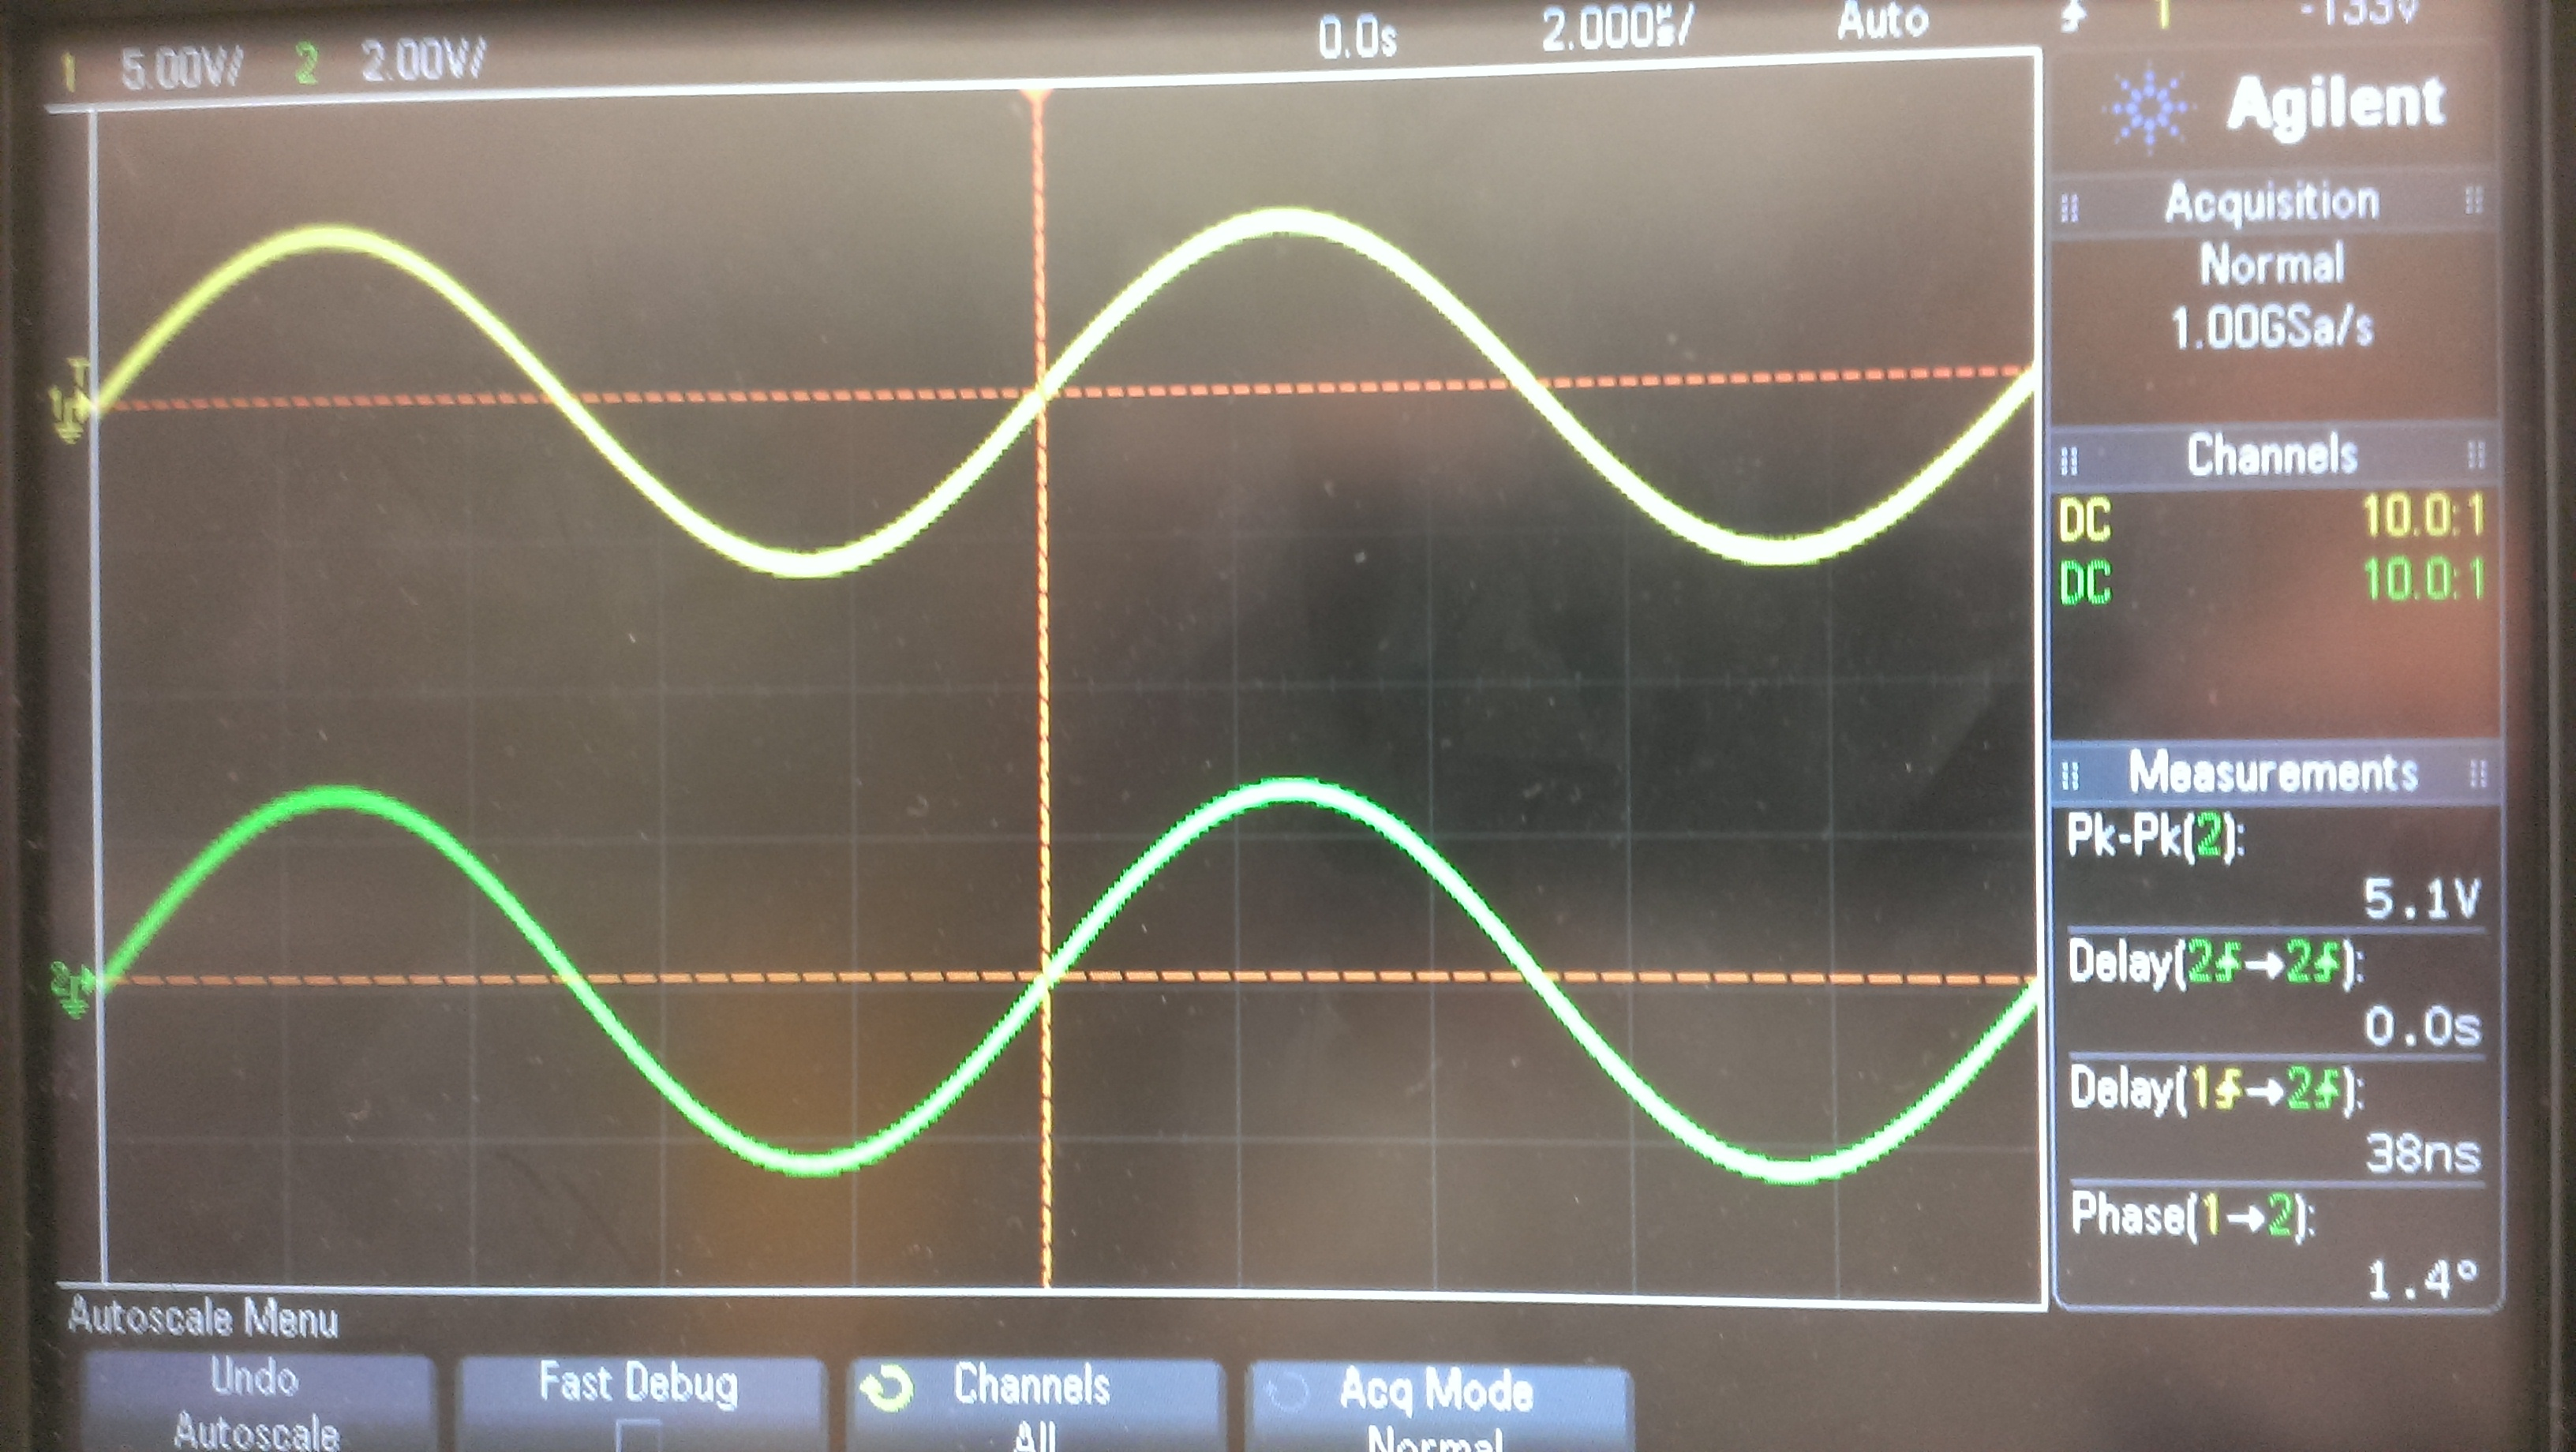
\includegraphics[width=0.8\textwidth]{./Images/RoleWave1.jpg}
    \caption{Oscilloscope output for a 100 kHz signal along a 12" cable}
\end{figure}
\begin{figure}[H]
    \centering
    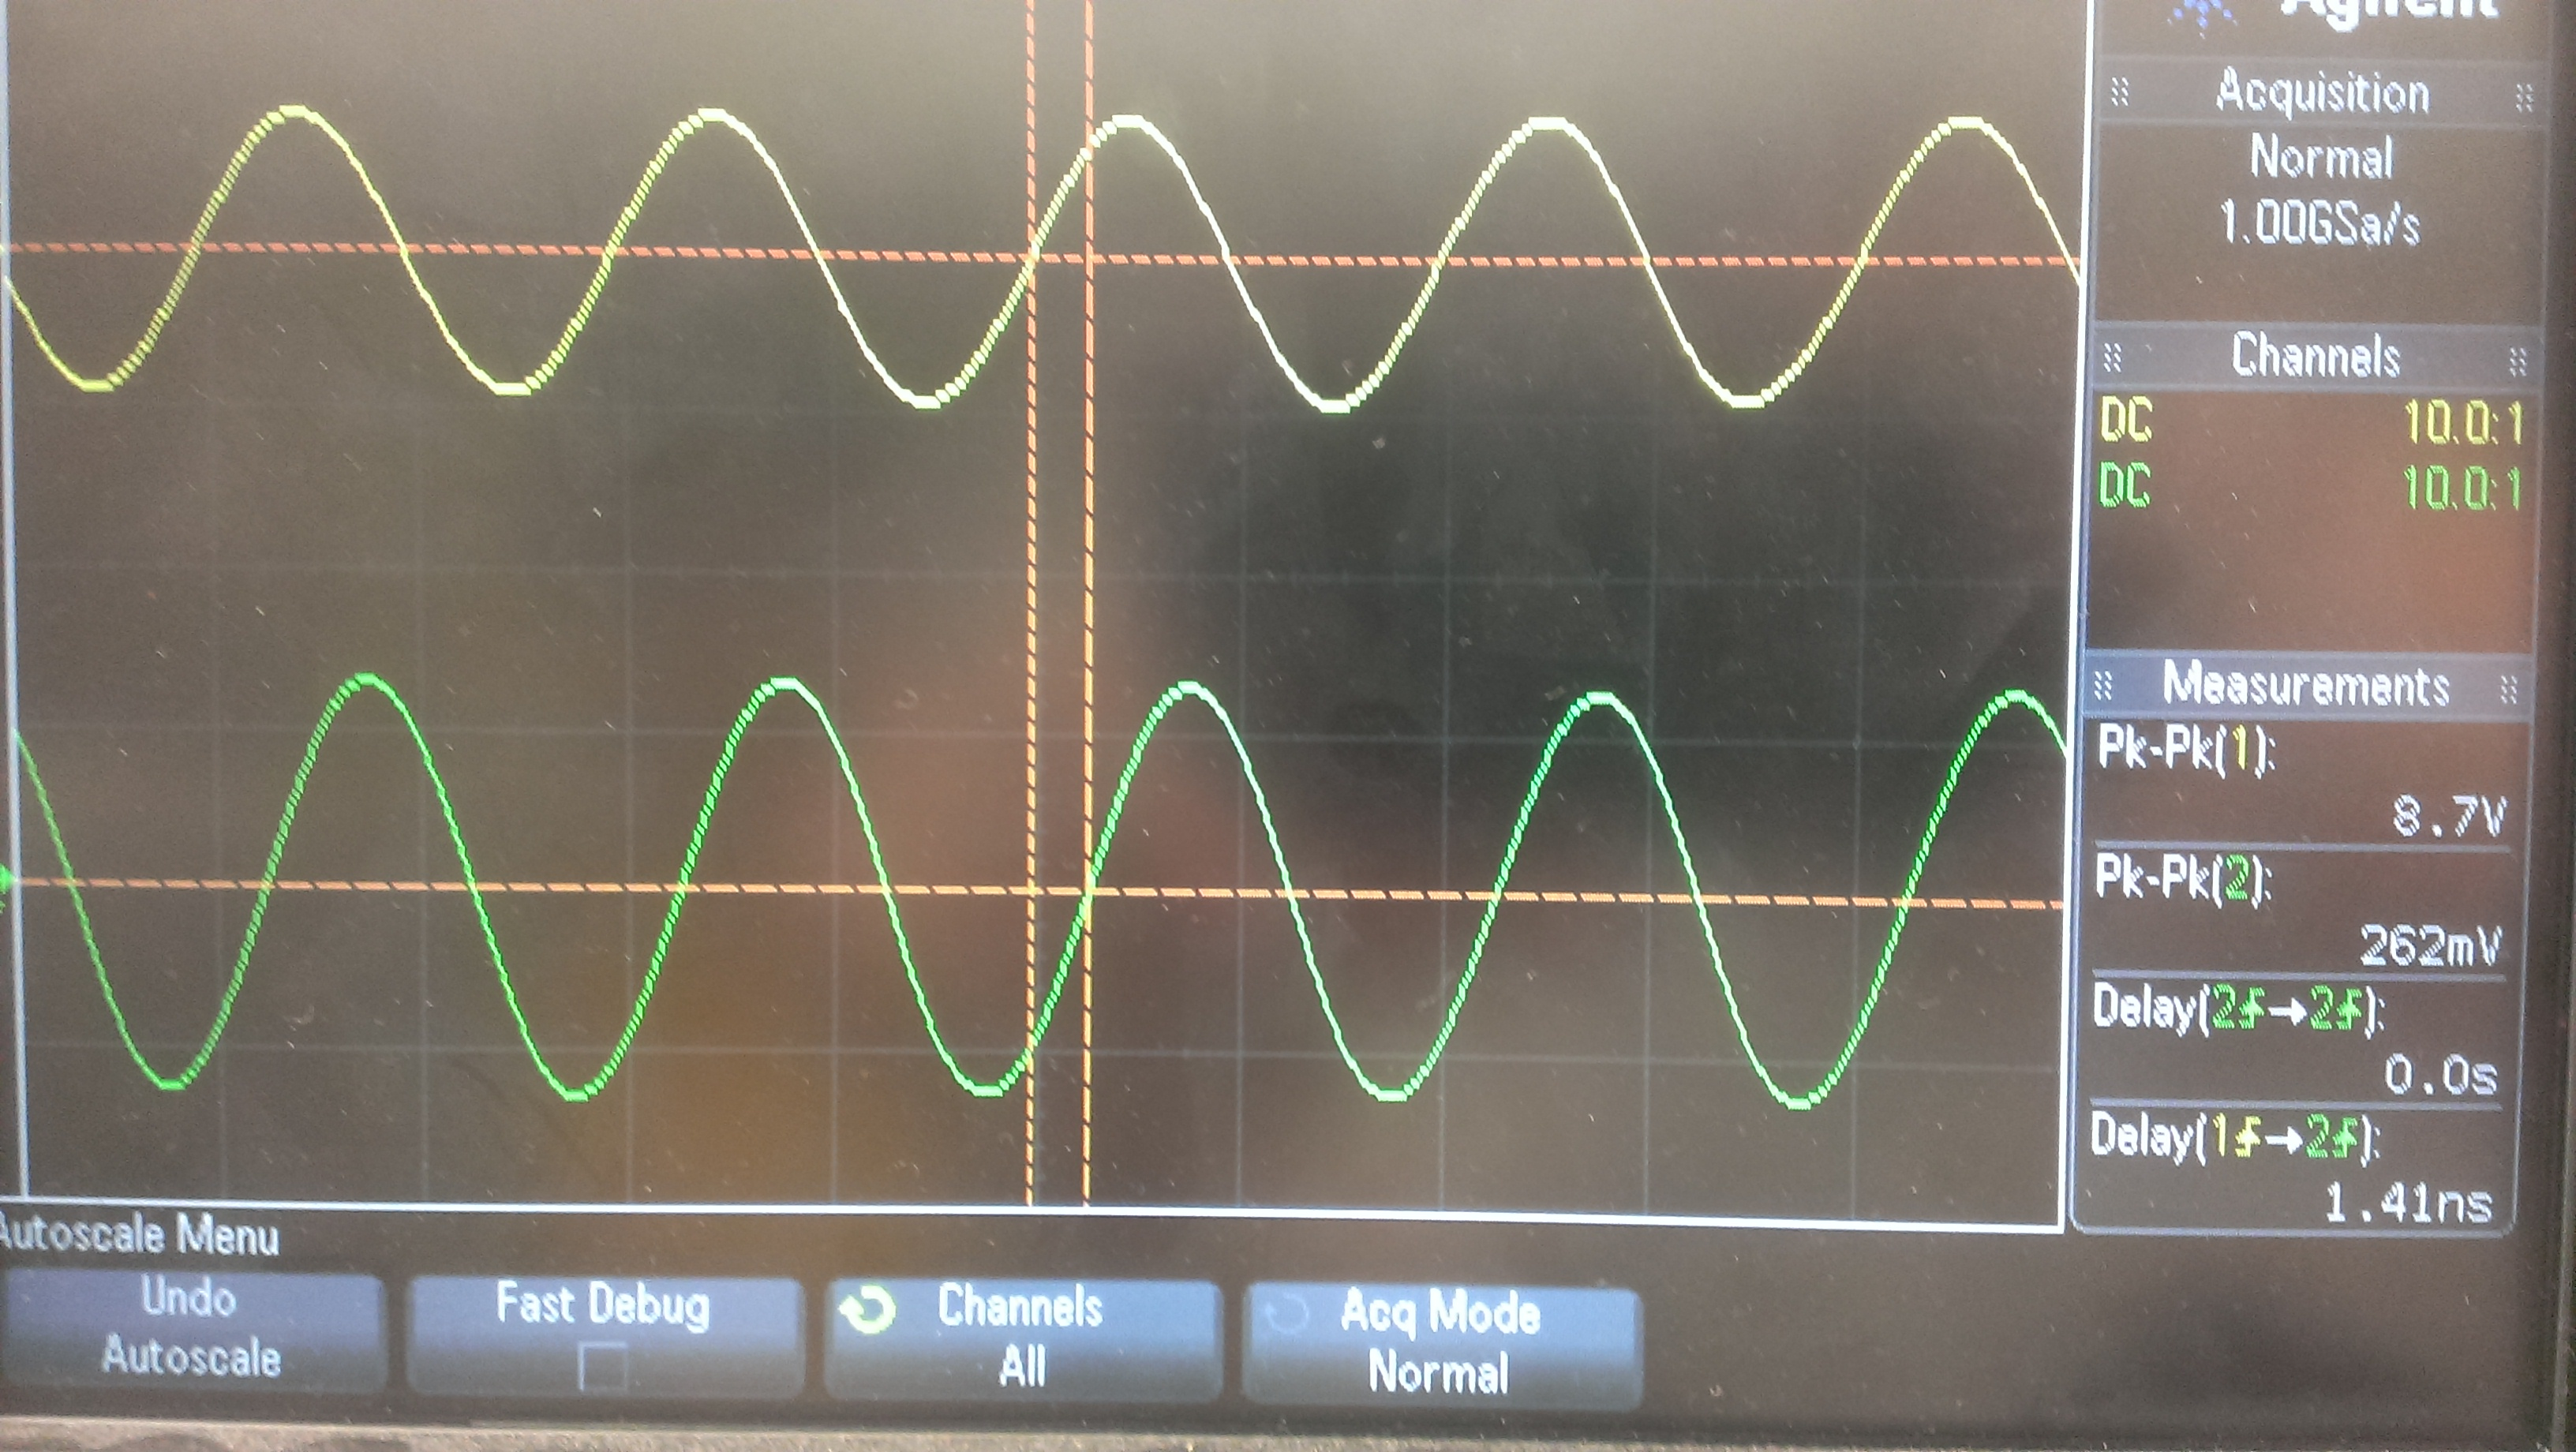
\includegraphics[width=0.8\textwidth]{./Images/RoleWave2.jpg}
    \caption{Oscilloscope output for a 100 kHz signal along a 180" cable}
\end{figure}
\begin{figure}[H]
    \centering
    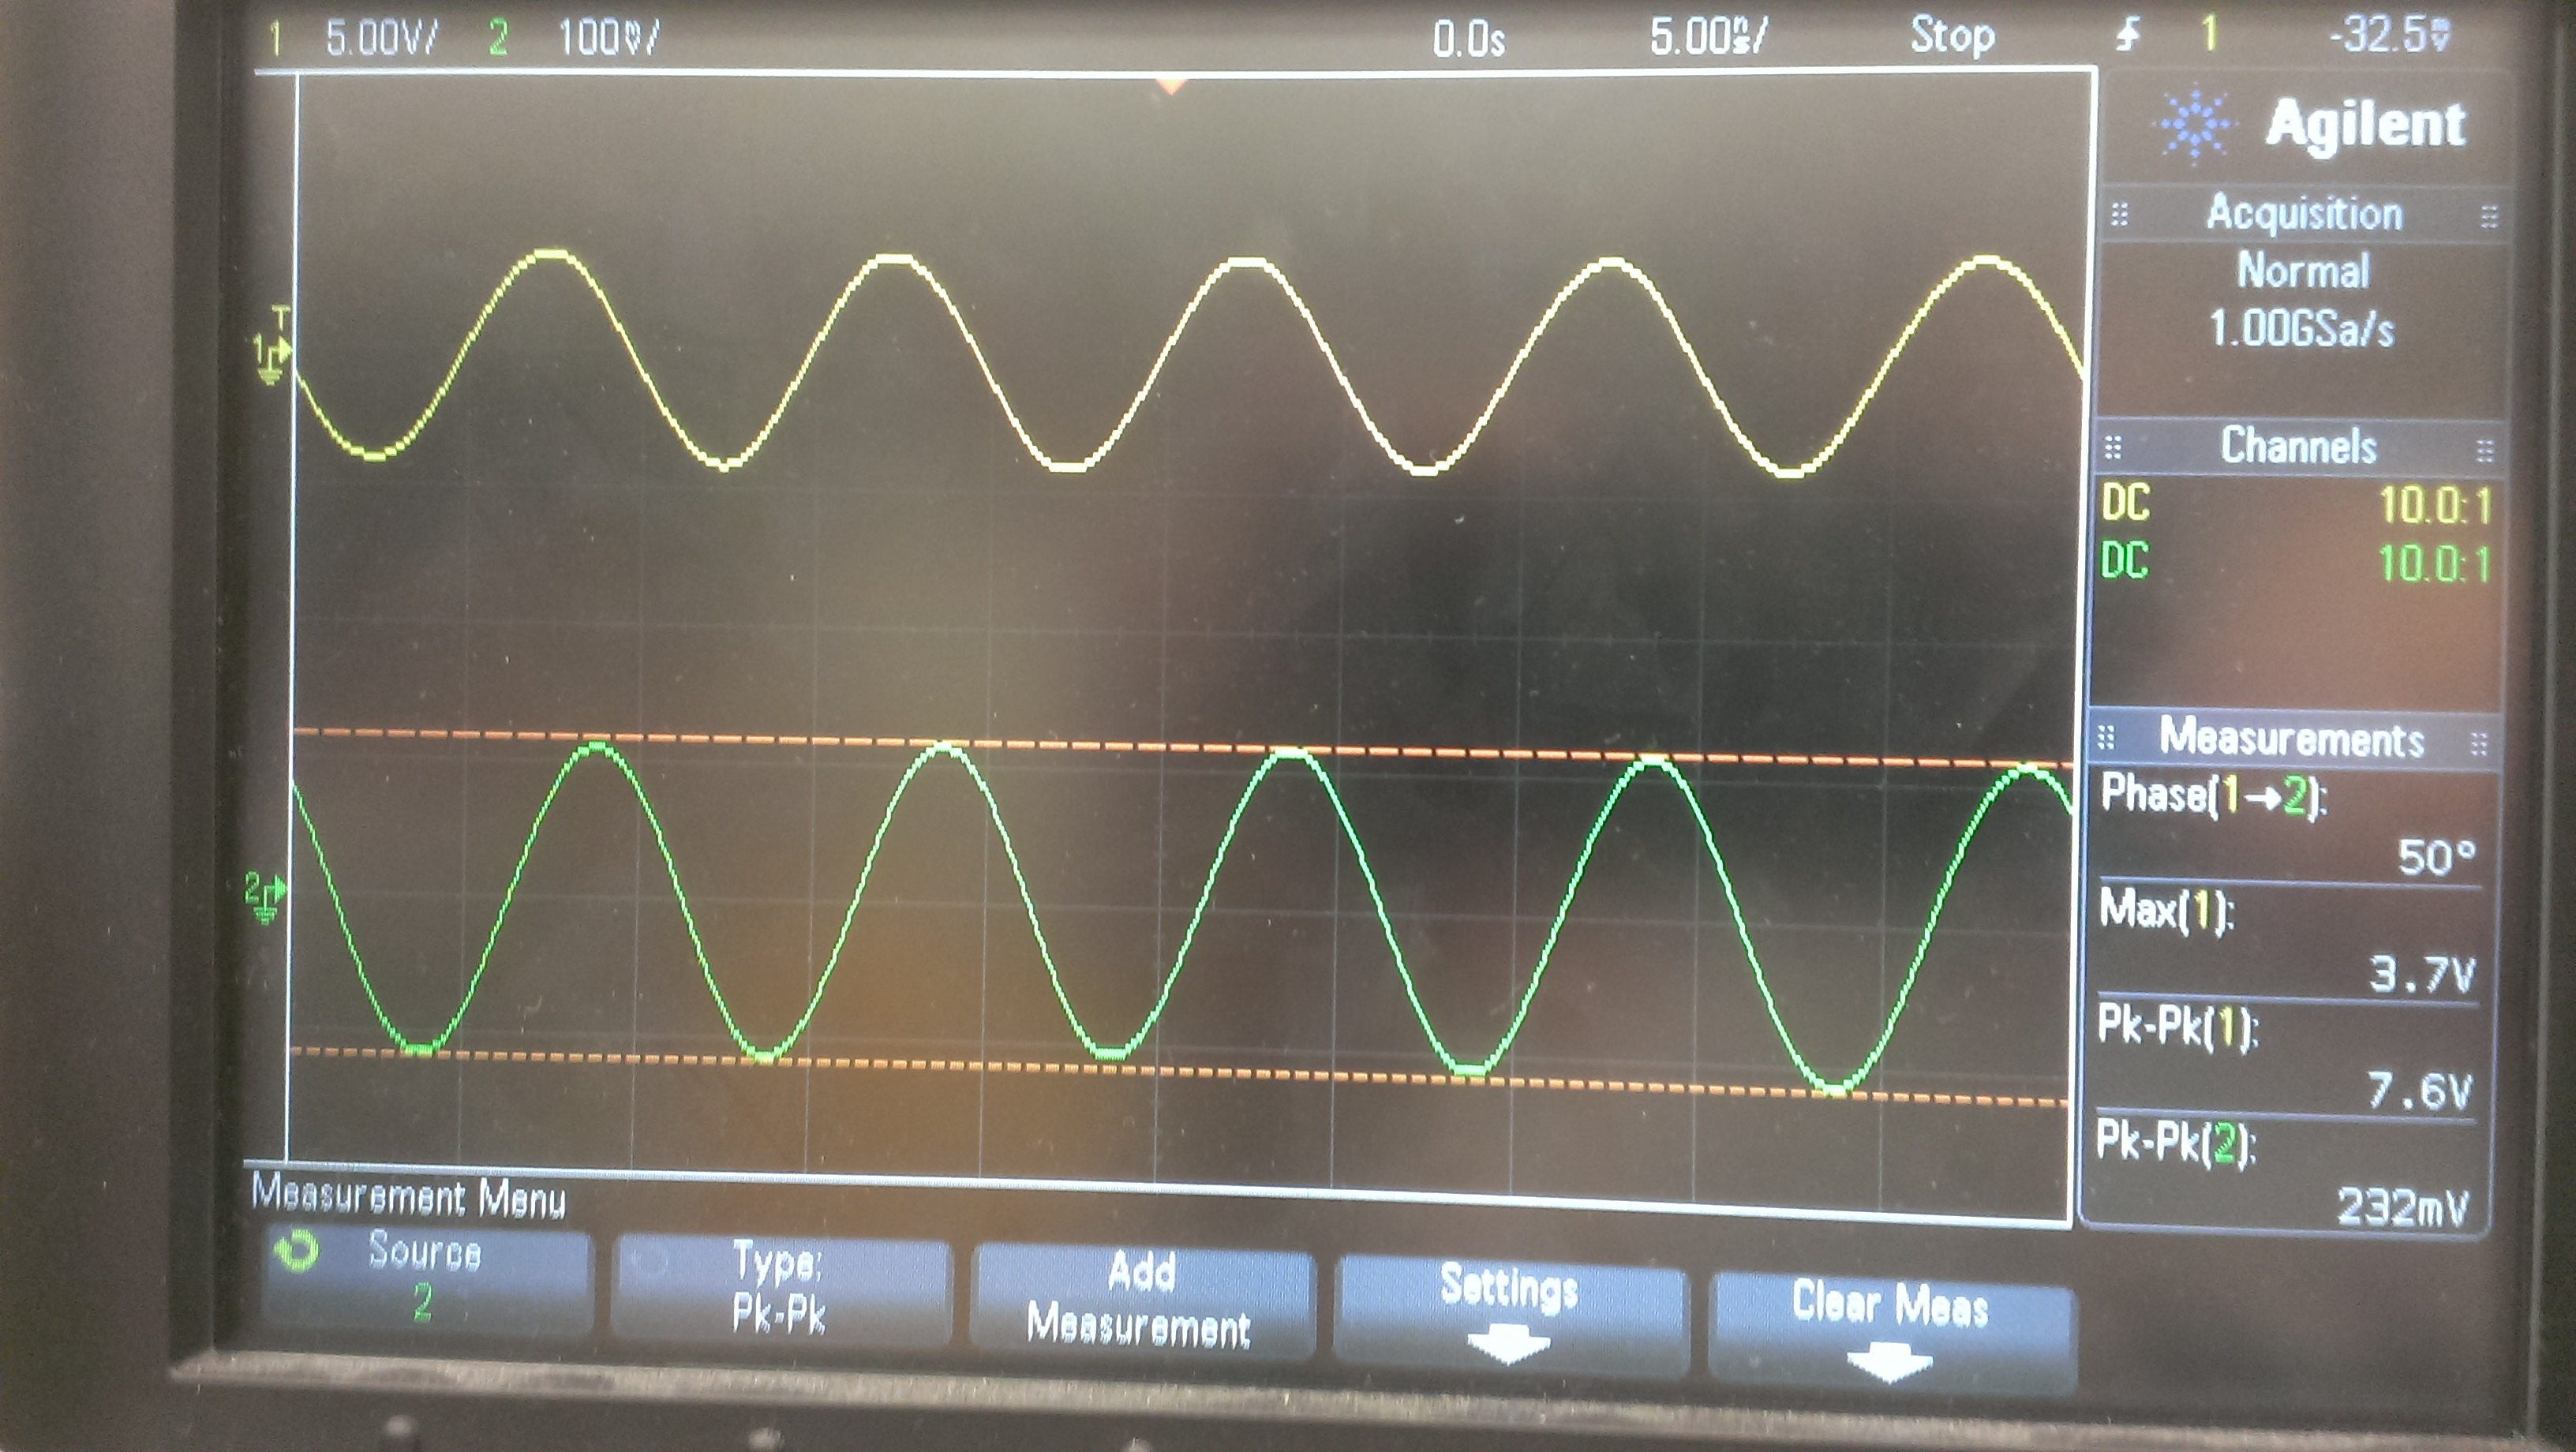
\includegraphics[width=0.8\textwidth]{./Images/RoleWave3.jpg}
    \caption{Oscilloscope output for a 100 MHz signal along a 12" cable}
\end{figure}
\begin{figure}[H]
    \centering
    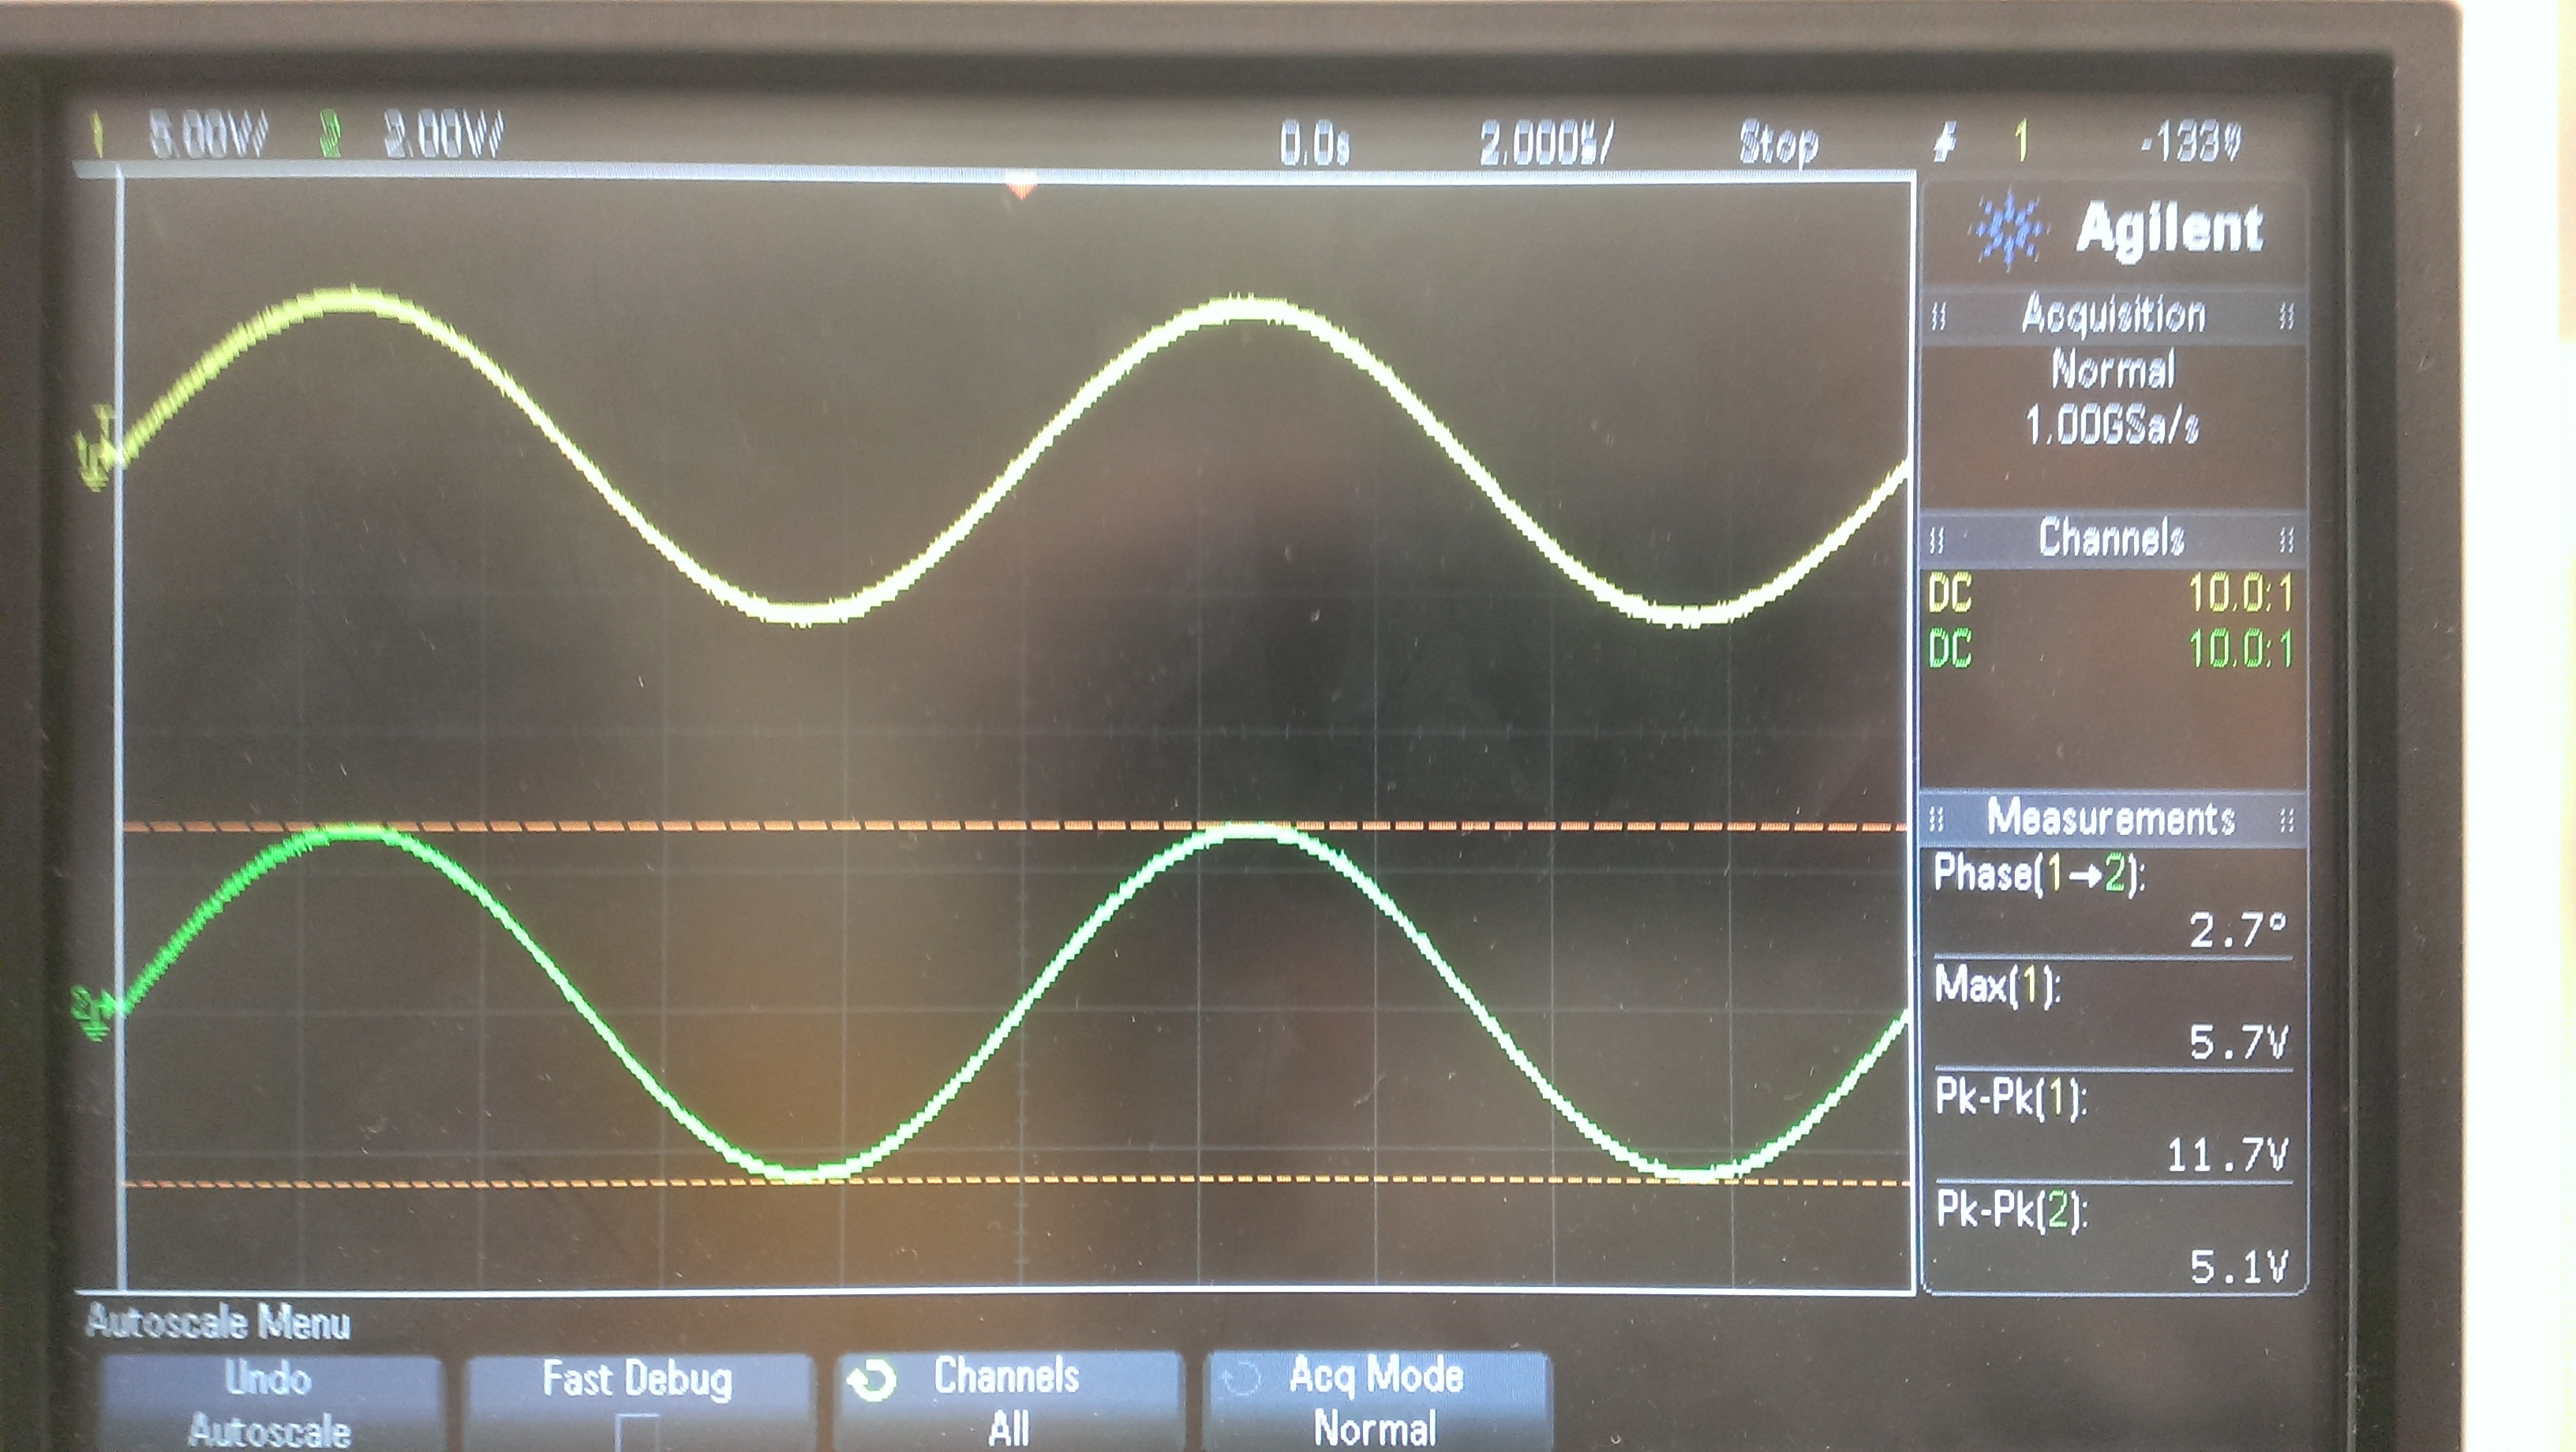
\includegraphics[width=0.8\textwidth]{./Images/RoleWave4.jpg}
    \caption{Oscilloscope output for a 100 MHz signal along a 180" cable}
\end{figure}
\begin{figure}[H]
    \centering
    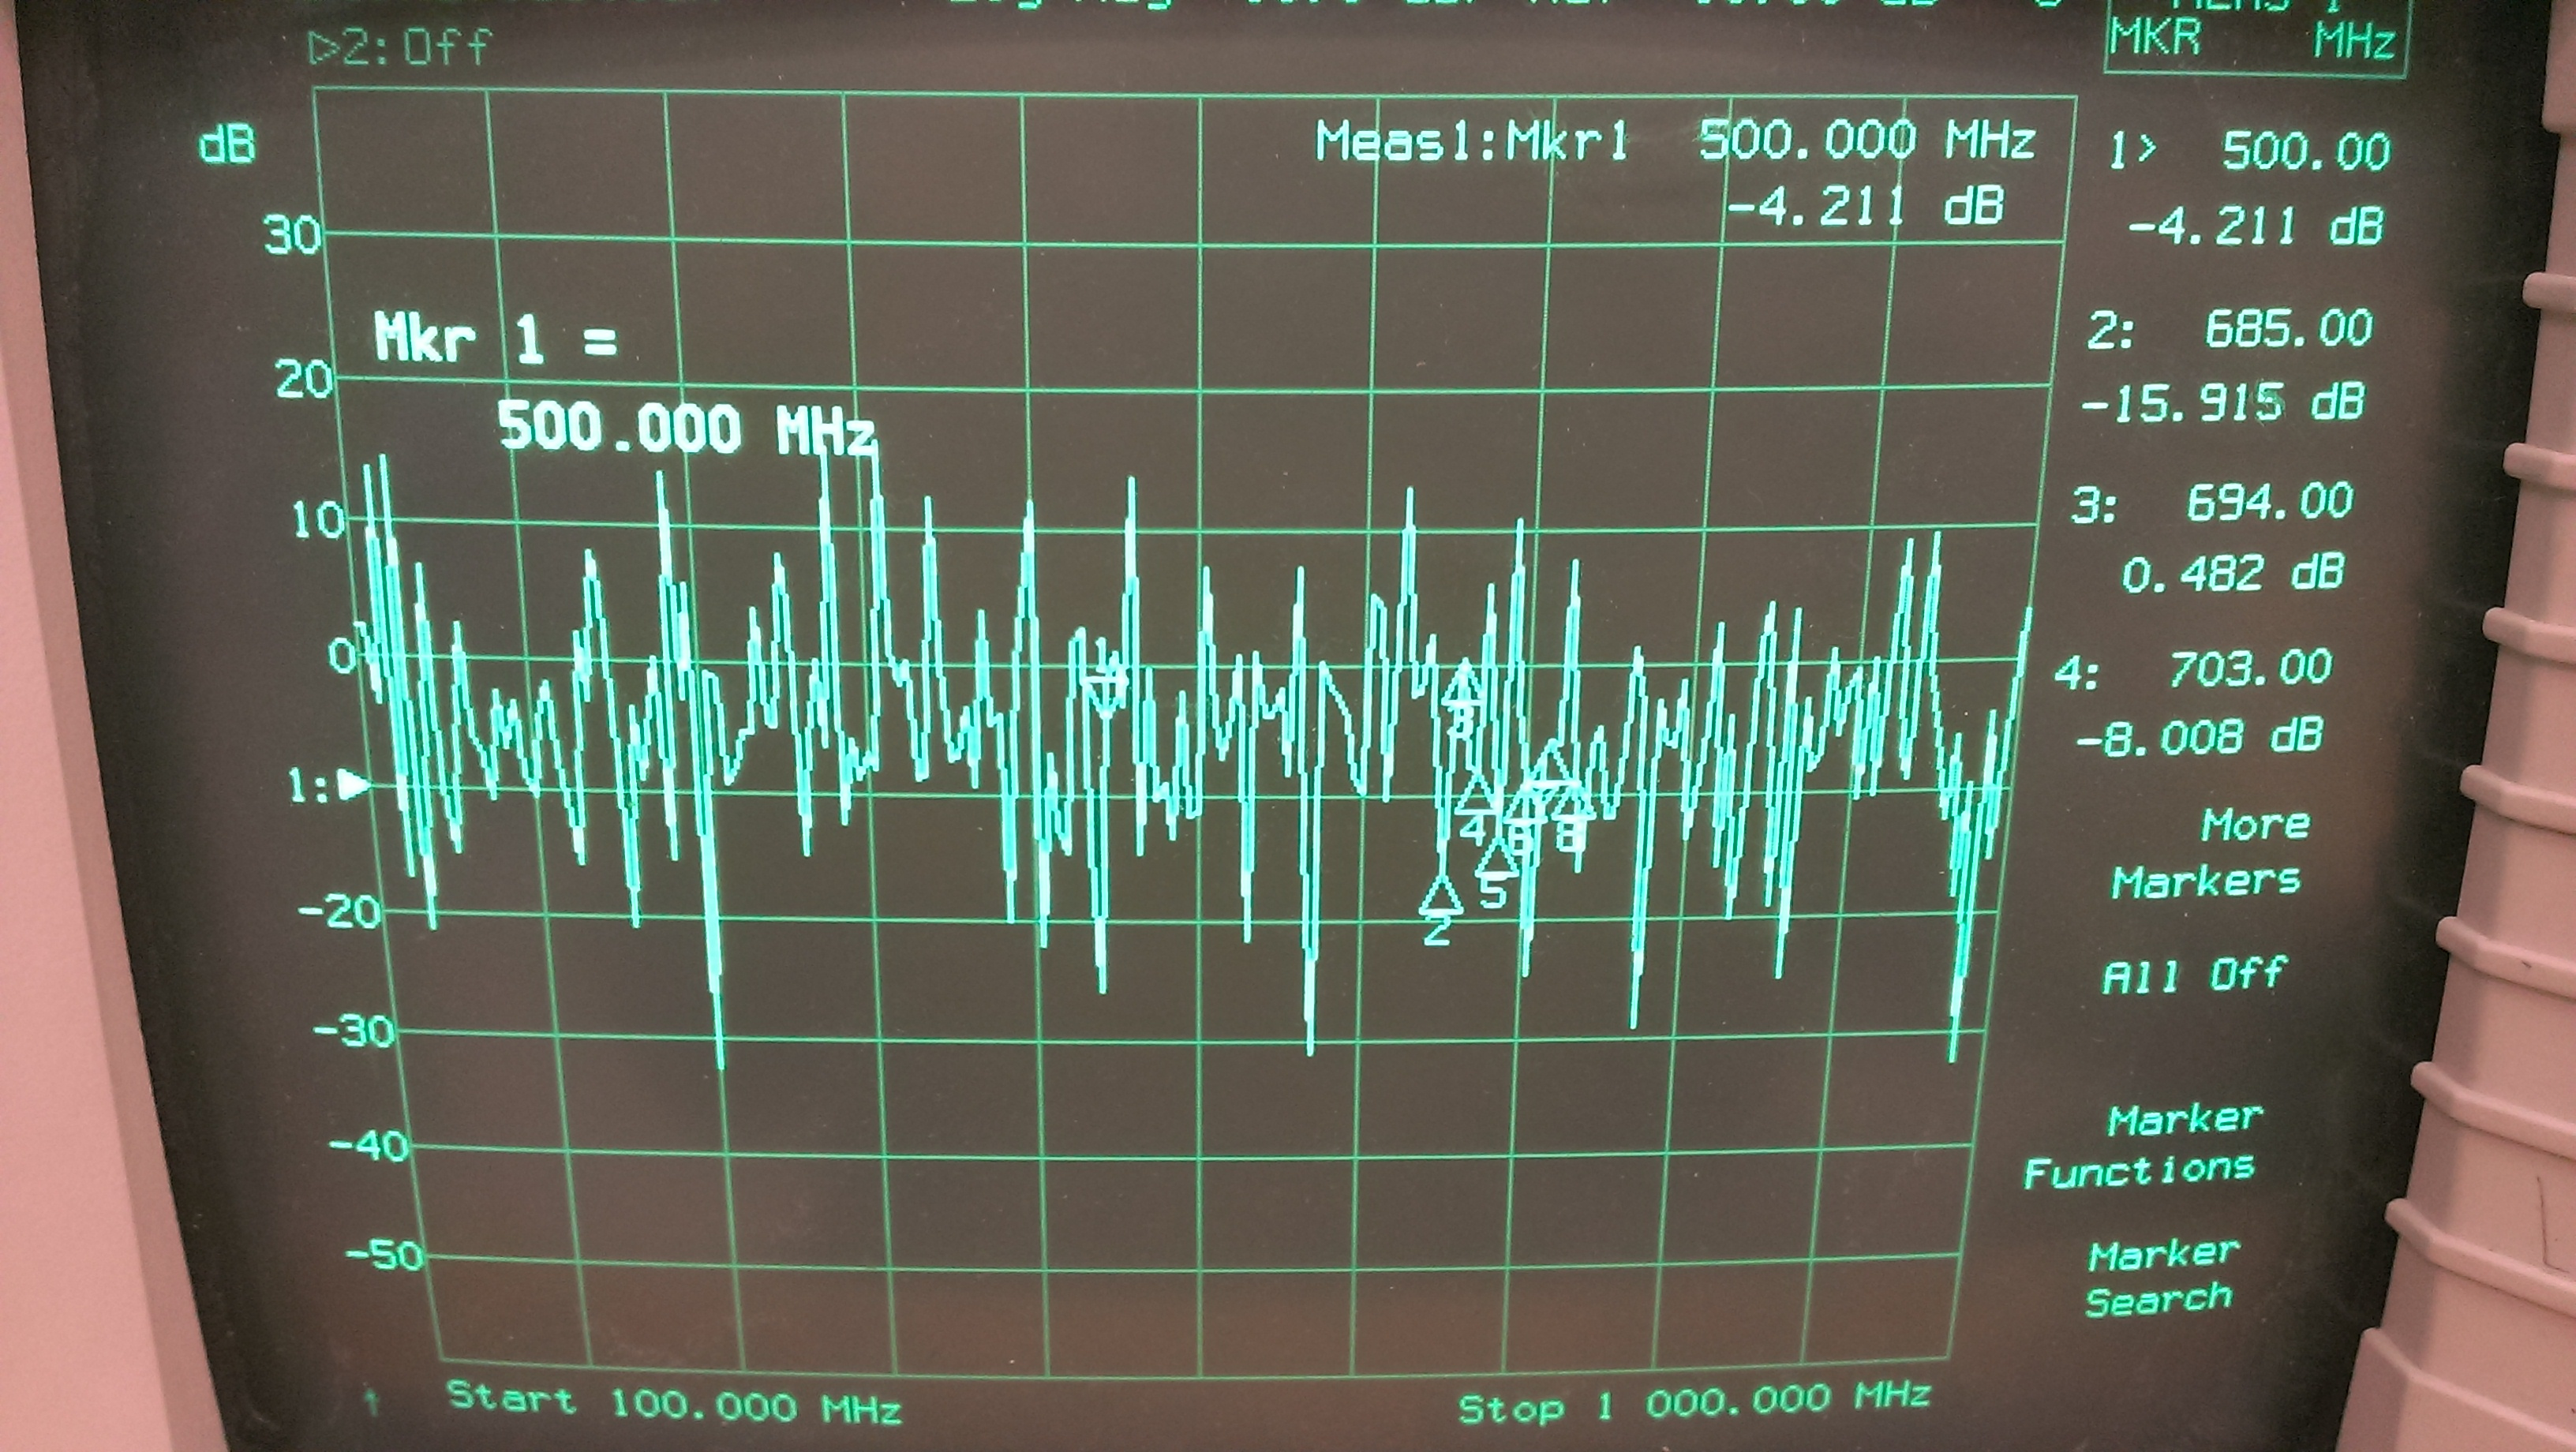
\includegraphics[width=0.8\textwidth]{./Images/NetShortUncal.jpg}
    \caption{Uncalibrated network analyzer output for a shorted load}
\end{figure}
\begin{figure}[H]
    \centering
    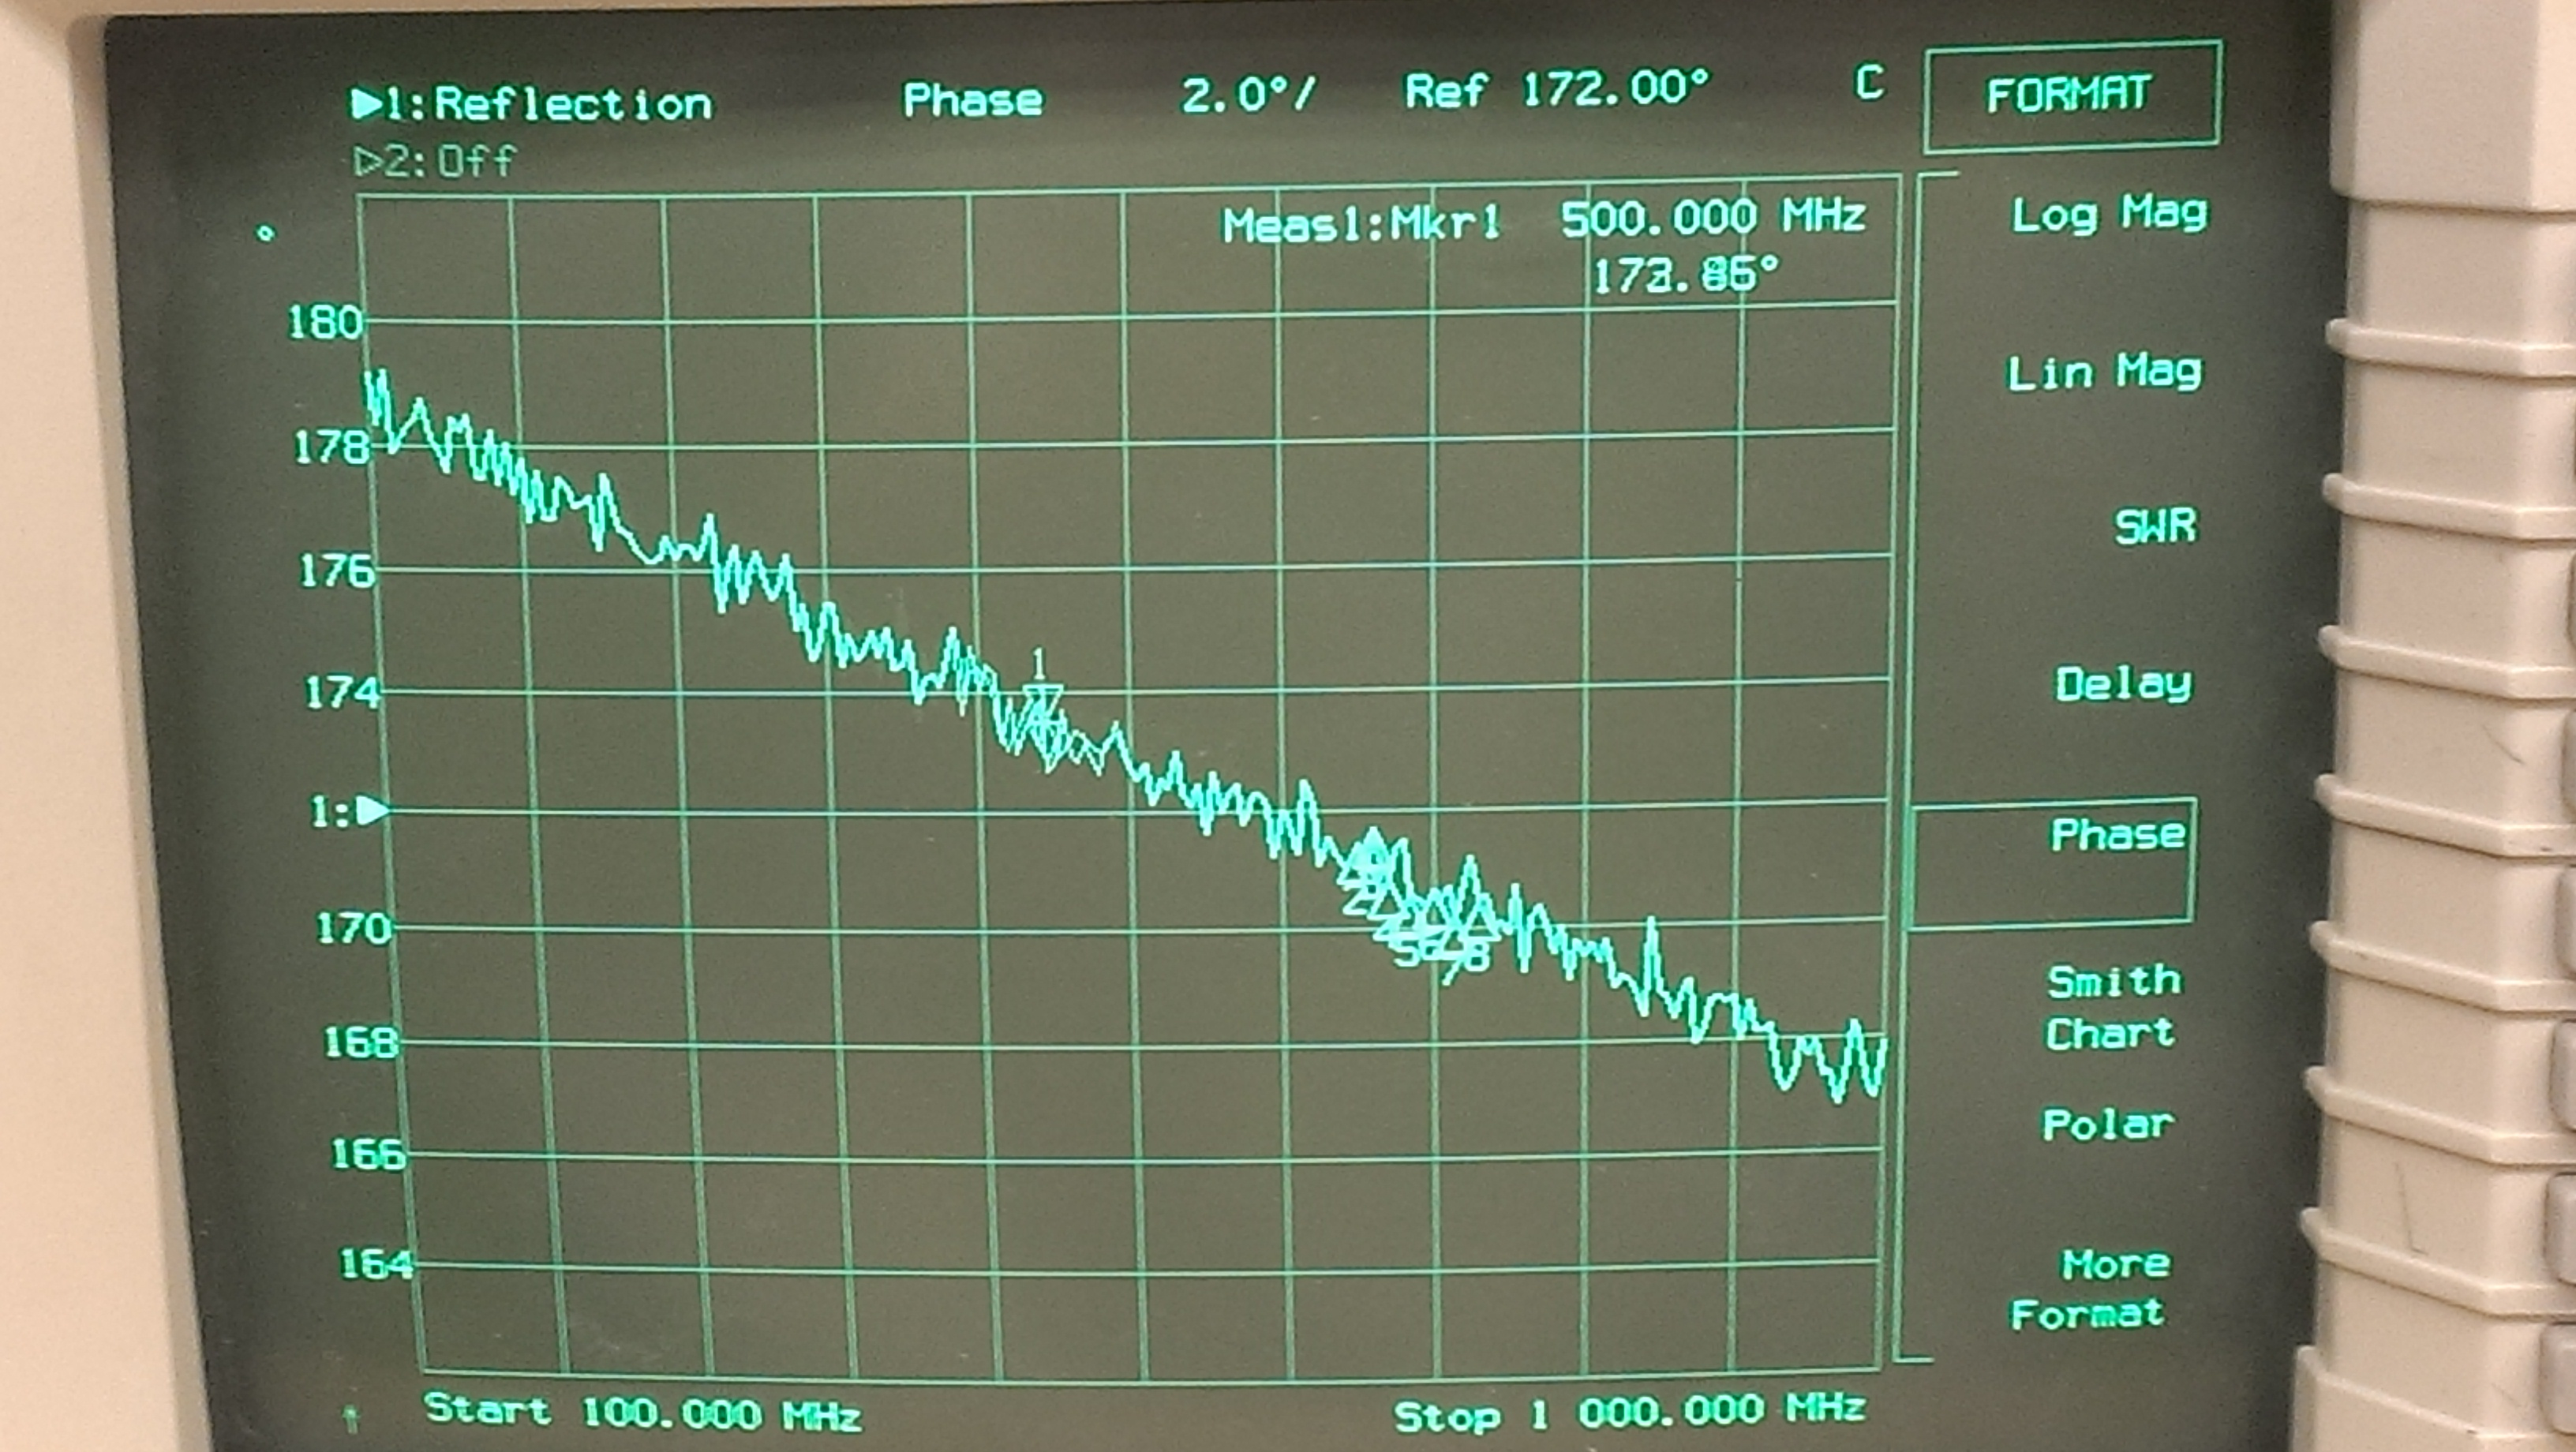
\includegraphics[width=0.8\textwidth]{./Images/NetShortCal.jpg}
    \caption{Calibrated network analyzer output for a shorted load}
\end{figure}
\begin{figure}[H]
    \centering
    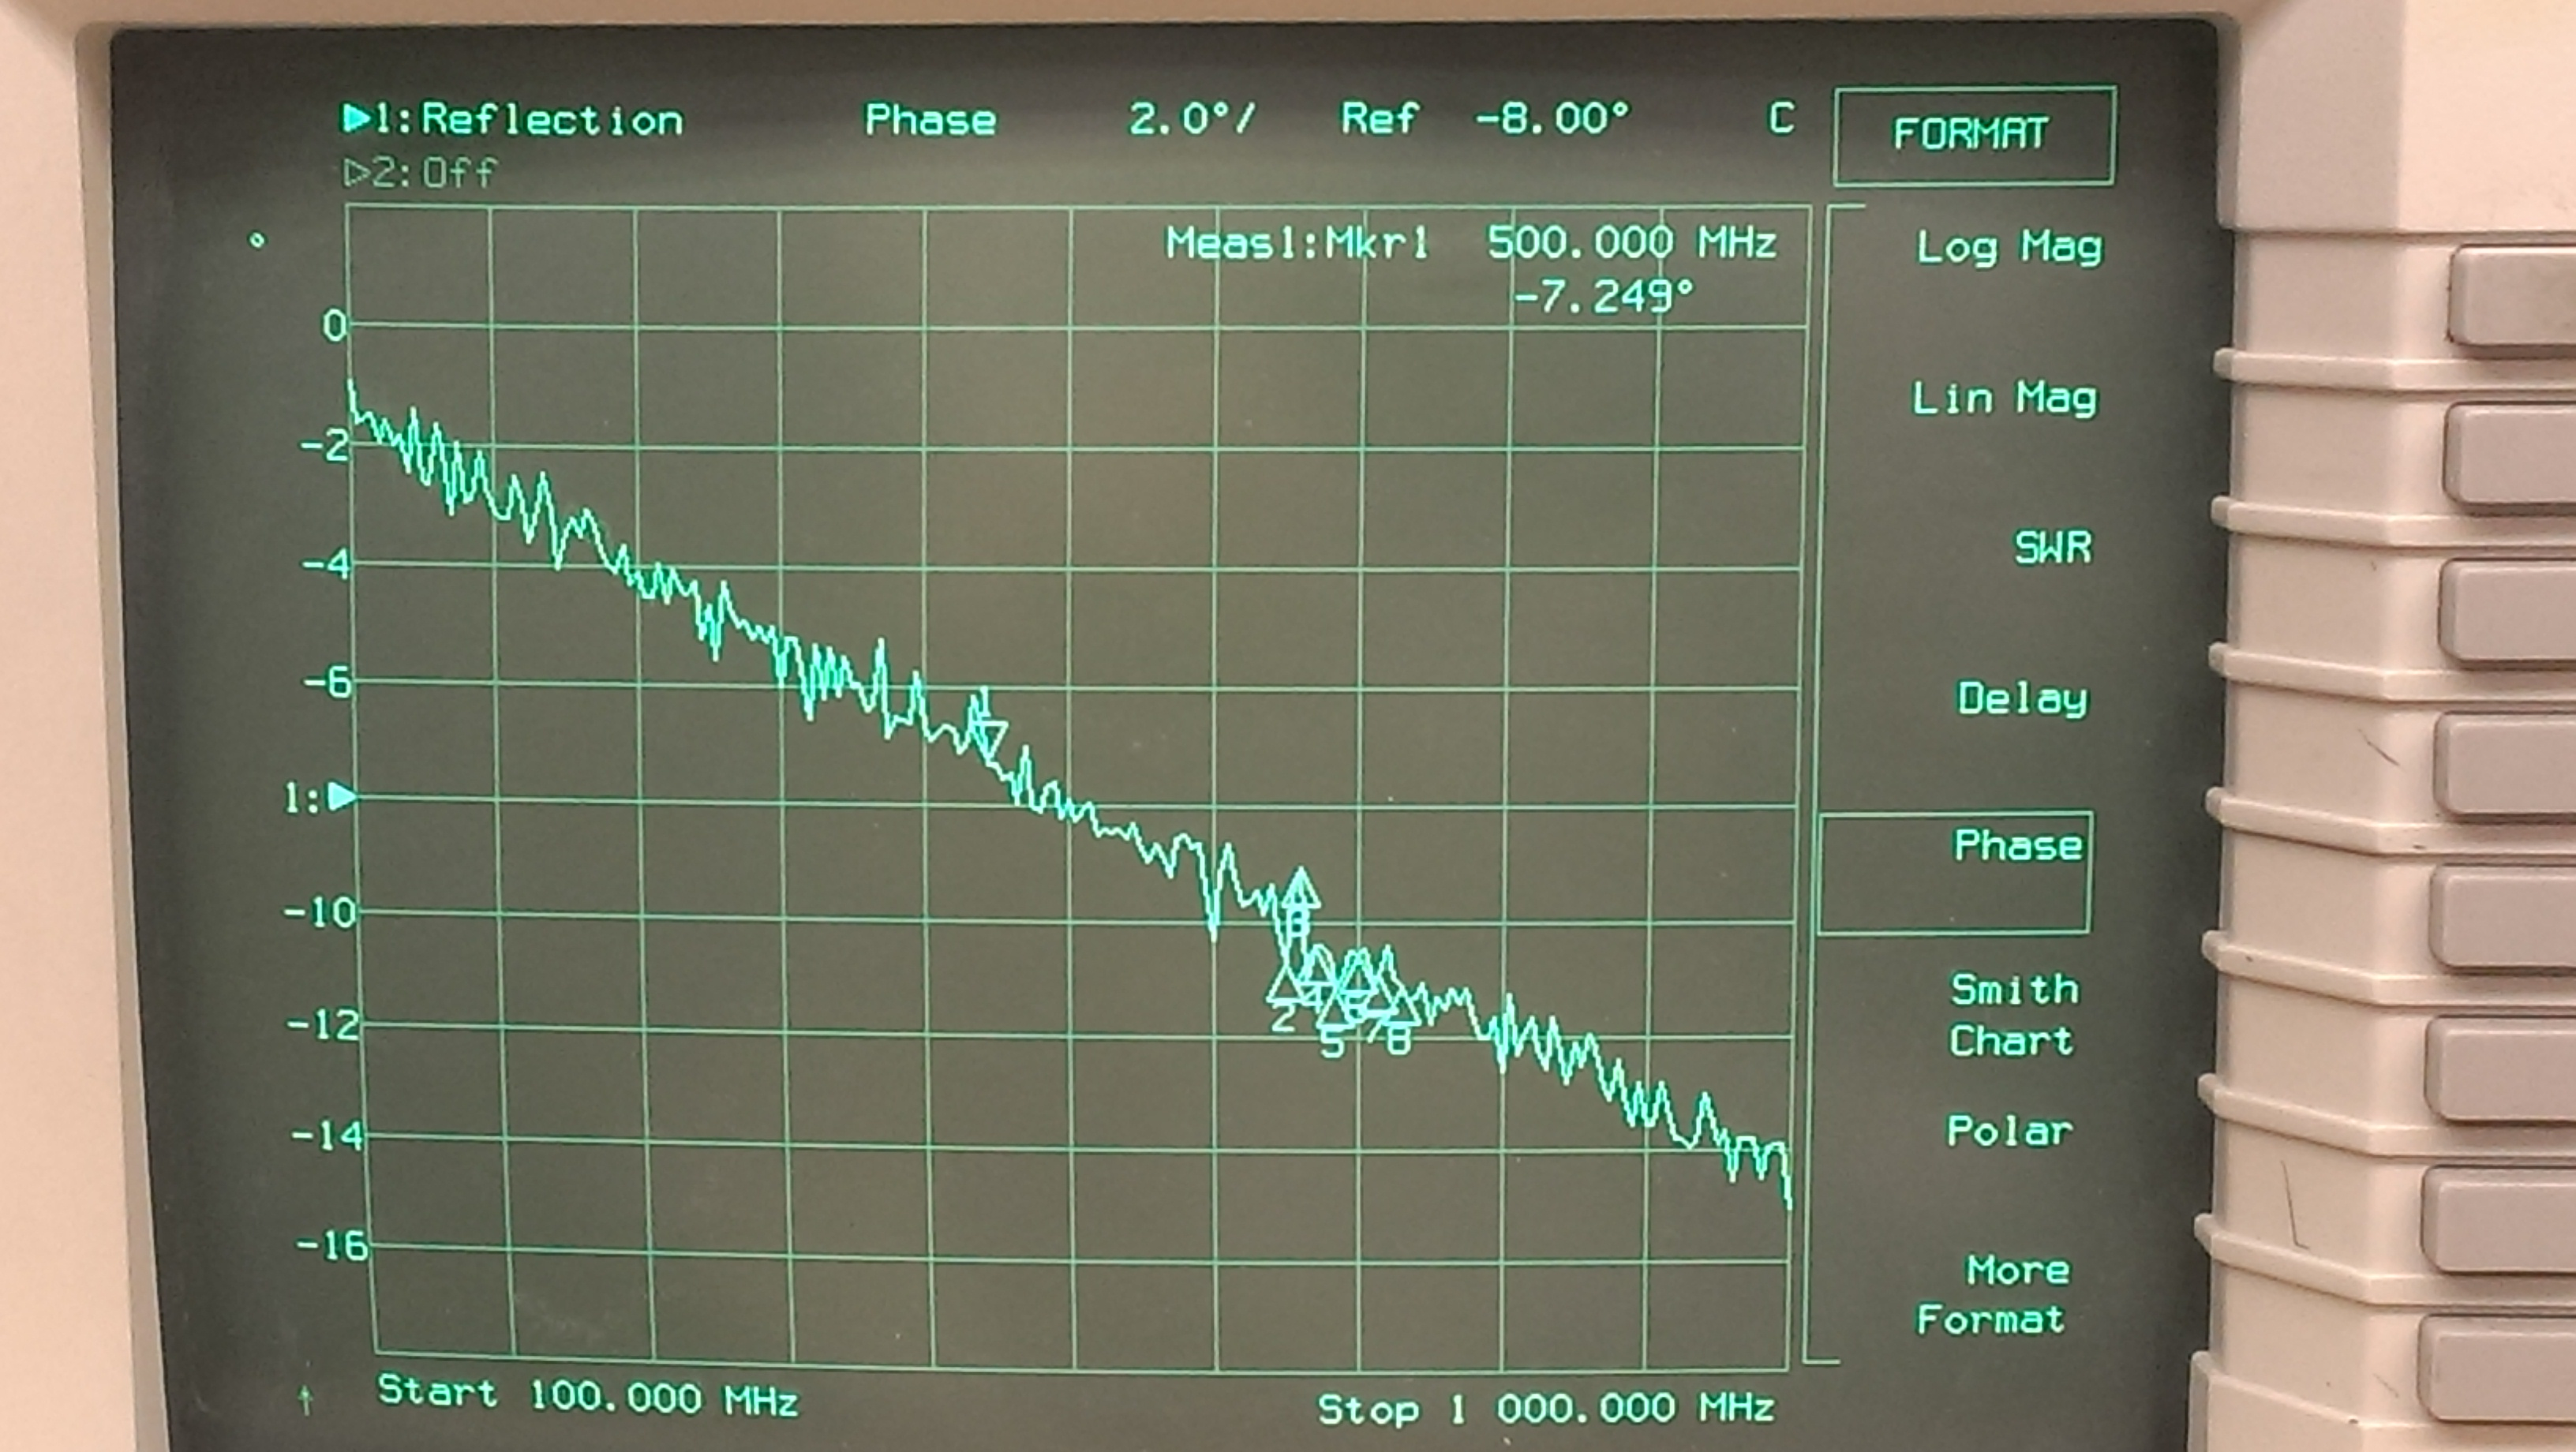
\includegraphics[width=0.8\textwidth]{./Images/NetOpen.jpg}
    \caption{Calibrated network analyzer output for a open load}
\end{figure}
\begin{figure}[H]
    \centering
    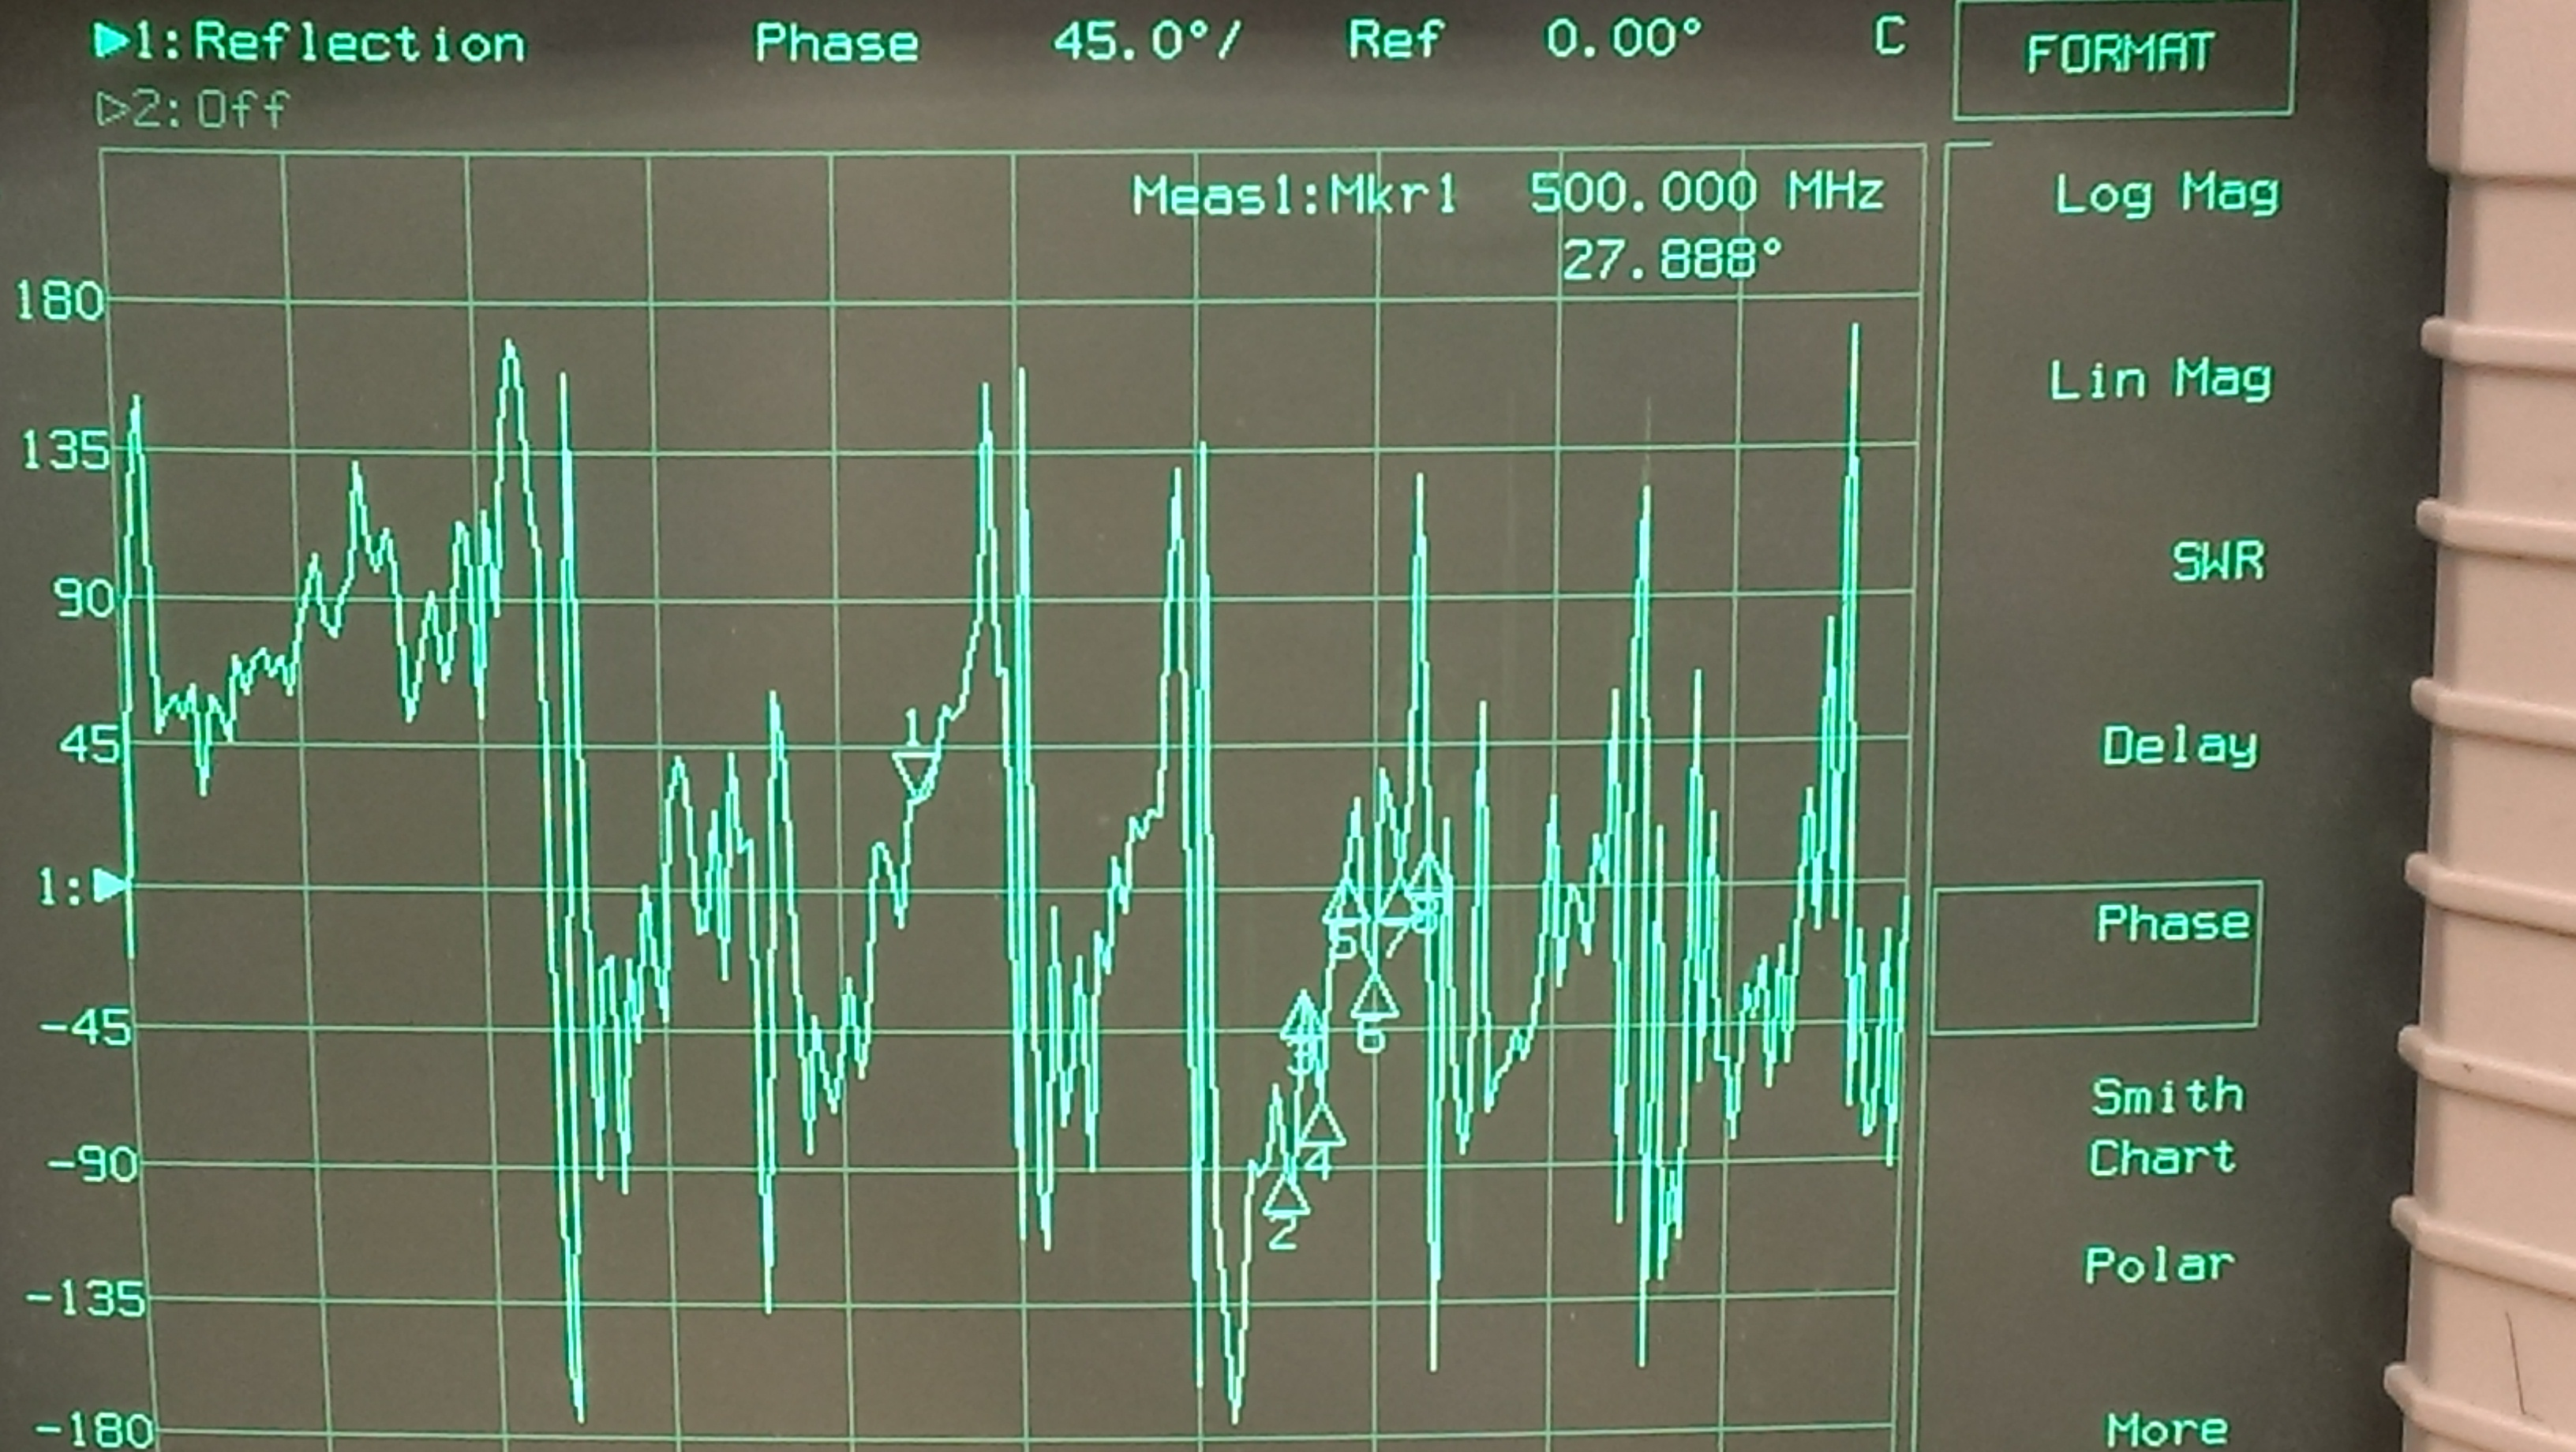
\includegraphics[width=0.8\textwidth]{./Images/NetMatch.jpg}
    \caption{Calibrated network analyzer output for a 50 $\Omega$ matched load}
\end{figure}
\begin{figure}[H]
    \centering
    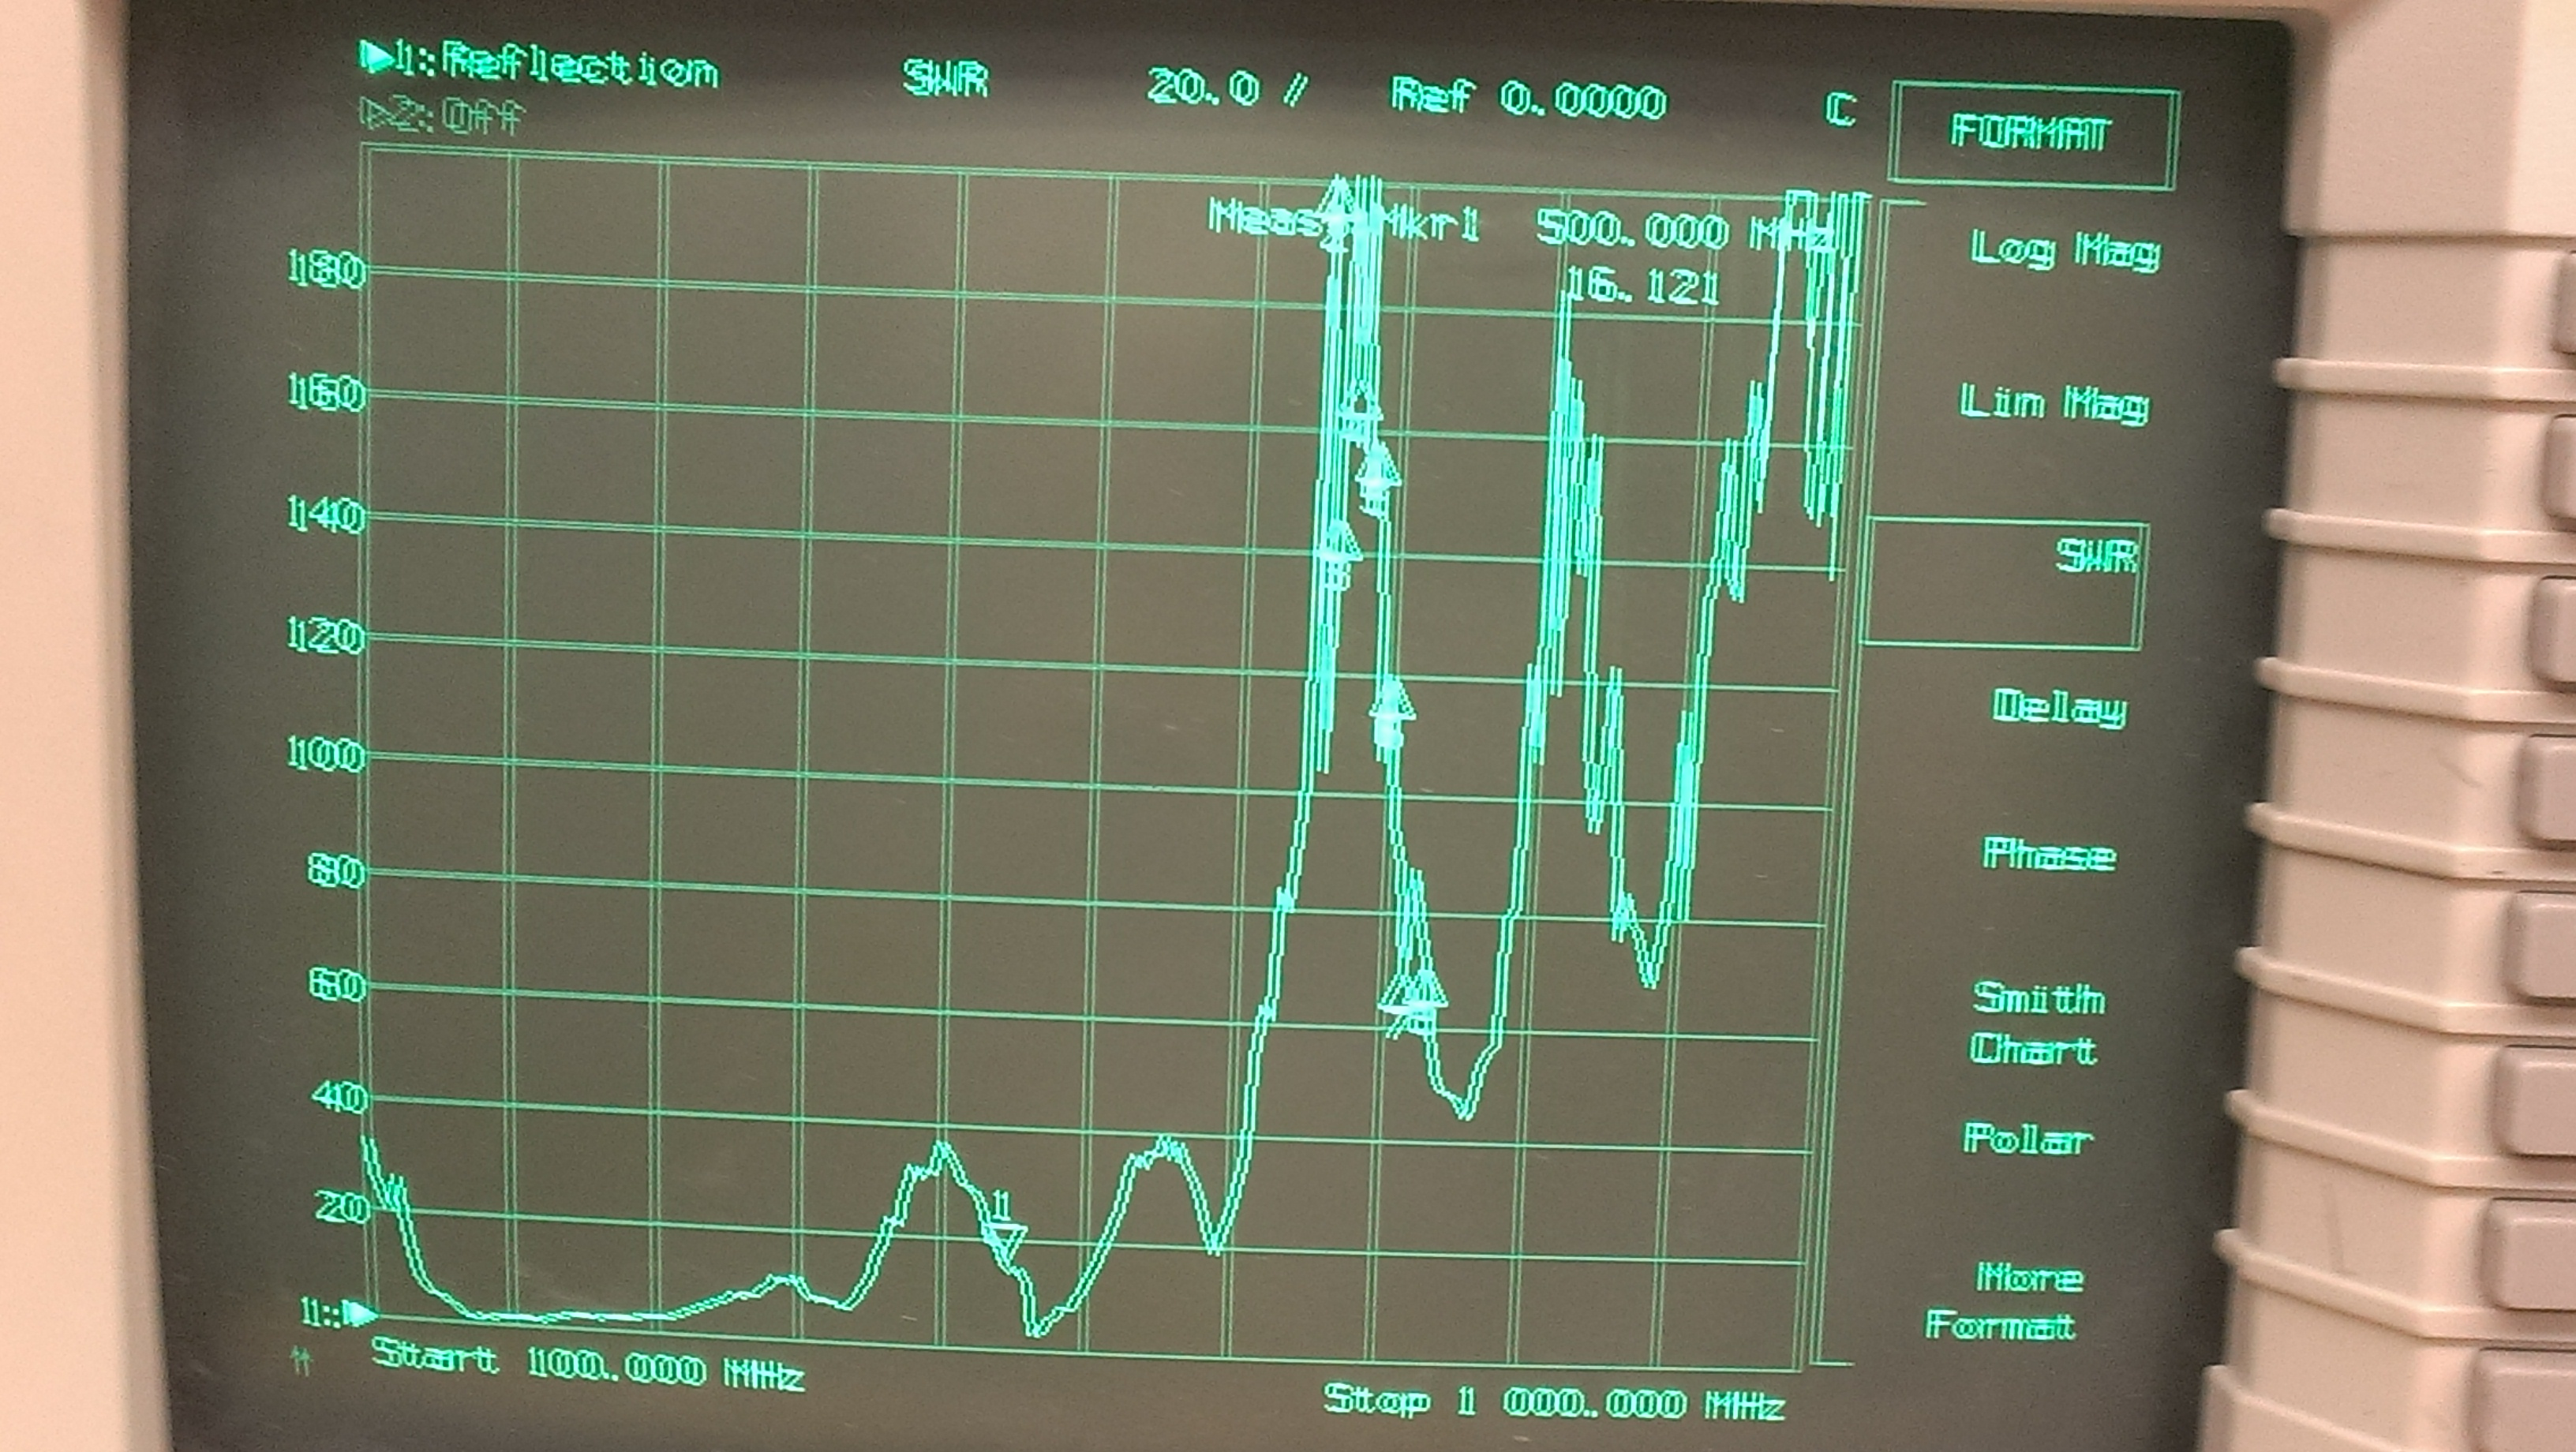
\includegraphics[width=0.8\textwidth]{./Images/NetSWR.jpg}
    \caption{Network analyzer output for the scanner antenna SWR}
\end{figure}

\end{document}